% \setchapterpreamble[u]{\margintoc}
\chapter{Essentials of Linux}
\labch{basic}

\section{Introduction}

\subsection{What is Linux?}

\begin{definition}[Linux]
  Linux is a \textbf{kernel} that is used in many operating systems. It is open source and free to use. Linux is not an operating system unto itself, but the core component of it.
\end{definition}

So what is \textbf{Ubuntu}? \textbf{Ubuntu} is one of the many \textit{distributions} that use the Linux kernel. It is a complete operating system that is free to use and open source. It is based on the \textbf{Debian} distribution of Linux. There are many other \textit{distributions} of Linux, such as:

\begin{itemize}
  \item
    \textbf{Debian} - Used primarily on servers, it is known for its stability.
    \begin{itemize}
      \item \textbf{Ubuntu} - A commercial distribution based on Debian which is popular among new users.
      \item \textbf{Linux Mint} - A distribution based on Ubuntu which is known for its ease of use. It is one of the distributions recommended to new users.
      \item \textbf{Pop OS} - A distribution based on Ubuntu which is known for its focus on developers, creators, and gamers.
      \item and many more
    \end{itemize}
  \item
    \textbf{Red Hat Enterprise Linux (RHEL)} - A commercial distribution used primarily in enterprises. It is owned by \textbf{Red Hat} and is targeted primarily to companies with their free OS paid support model.
    \begin{itemize}
      \item \textbf{Fedora} - A community-driven distribution sponsored by \textbf{Red Hat}. It is known for its cutting-edge features and is used by developers. It remains on the upstream of \textbf{RHEL}, receiving new features before \textbf{RHEL}.
      \item \textbf{CentOS} - A discontinued distribution based on \textbf{RHEL}. It was known for its stability and was used in servers. It was downstream from \textbf{RHEL}.
      \item \textbf{CentOS Stream} - It is a midstream between the upstream development in Fedora Linux and the downstream development for Red Hat Enterprise Linux.
      \item \textbf{Rocky Linux} - A distribution created by the \textbf{Rocky Enterprise Software Foundation} after the announcement of discontinuation of \textbf{CentOS}. It is a downstream of \textbf{RHEL} that provides feature parity and binary compatibility with \textbf{RHEL}.
      \item \textbf{Alma Linux} - A distribution created by the \textbf{CloudLinux} team after the announcement of discontinuation of \textbf{CentOS}. It is a downstream of \textbf{RHEL} that provides feature parity and binary compatibility with \textbf{RHEL}.
    \end{itemize}
  \item
    \textbf{Arch Linux} - A community-driven distribution known for its simplicity and customizability. It is a \textit{rolling release} distribution, which means that it is continuously updated. It is a bare-bones distribution that lets the user decide which packages they want to install.
    \begin{itemize}
      \item \textbf{Manjaro} - A distribution based on Arch Linux which is known for its user-friendliness. It is a rolling release distribution that is easier to install for new users. It uses a different repository for packages with additional testing.
      \item \textbf{EndeavourOS} - A distribution based on Arch Linux which is known for its simplicity and minimalism. It is a rolling release distribution that is easier to install for new users. It uses the same repository for packages as \textbf{Arch Linux}.
      \item \textbf{Artix Linux} - It uses the \textbf{OpenRC} init system instead of \textbf{systemd}. It also offers other \textit{init systems} like \textbf{runit}, \textbf{s6}, \textbf{dinit}.
    \end{itemize}
  \item
    \textbf{openSUSE} - It is a free and open-source Linux distribution developed by the openSUSE project. It is offered in two main variations: \textbf{Tumbleweed}, an upstream rolling release distribution, and \textbf{Leap}, a stable release distribution which is sourced from SUSE Linux Enterprise.
    \begin{itemize}
      \item \textbf{Tumbleweed} - Rolling Release upstream.
      \item \textbf{Leap} - Stable Release downstream.
    \end{itemize}
  \item
    \textbf{Gentoo} - A distribution known for its customizability and performance. It is a source-based distribution, which means that the user compiles the software from source code. It is known for its performance optimizations for the user's hardware.
  \item
    \textbf{Void} - It is an independent rolling-release Linux distribution that uses the X Binary Package System package manager, which was designed and implemented from scratch, and the \textbf{runit} init system. Excluding binary kernel blobs, a base install is composed entirely of free\sidenote{
      “Free software” means software that respects users' freedom and community. Roughly, it means that the users have the freedom to run, copy, distribute, study, change and improve the software. Thus, “free software” is a matter of liberty, not price. To understand the concept, you should think of “free” as in “free speech,” not as in “free beer.” We sometimes call it “libre software,” borrowing the French or Spanish word for “free” as in freedom, to show we do not mean the software is gratis. \\\\ You may have paid money to get copies of a free program, or you may have obtained copies at no charge. But regardless of how you got your copies, you always have the freedom to copy and change the software, even to sell copies. \\\\ - \href{https://www.gnu.org/philosophy/free-sw.en.html}{GNU on Free Software}
    } software.
\end{itemize}

\begin{marginfigure}
	\includegraphics{dist-chart}
	\caption[Linux Distributions Usage]{Linux Distributions Usage in 2024}
	\labfig{dist-chart}
\end{marginfigure}

\subsection{Desktop Environments}
\begin{definition}[Desktop Environment]
  A desktop environment is a collection of software designed to give functionality and a certain look and feel to a desktop operating system. It is a combination of a window manager, a file manager, a panel, and other software that provides a graphical user interface and utilities to a regular desktop user, such as volume and brightness control, multimedia applications, settings panels, etc. This is only required by desktop (and laptop) uses and are not present on server instances.
\end{definition}

There are many desktop environments available for Linux, but the important ones are:

\begin{itemize}
  \item
    \textbf{GNOME} - One of the most popular desktop environments for Linux. It is known for its simplicity and ease of use. It is the default desktop environment for many distributions, including Ubuntu. It is based on the \textbf{GTK} Toolkit.
    \sidenote{GTK is a free software cross-platform widget toolkit for creating graphical user interfaces.}
    Popular distros shipping by default with GNOME are Fedora, RHEL, CentOS, Debian, Zorin, and Ubuntu.
    \sidenote{Ubuntu used to ship with Unity as the default desktop environment, but switched to GNOME in 2017.}
  \item
    \textbf{KDE Plasma} - A highly customizable desktop environment based on the \textbf{Qt} Tookit.
    \sidenote{Qt is cross-platform application development framework for creating graphical user interfaces.}
    Many distributions like Slackware and OpenSUSE ship with KDE Plasma as the default desktop environment, and most others have the option to install with KDE Plasma. Ubuntu's KDE Plasma variant is called \textbf{Kubuntu}.
  \item
    \textbf{Xfce} - A lightweight desktop environment known for its speed and simplicity. It is based on the \textbf{GTK} Toolkit. It is used in many distributions like Xubuntu, Manjaro, and Fedora.
  \item
    \textbf{LXQt} - A lightweight desktop environment known for its speed and simplicity. It is based on the \textbf{Qt} Toolkit. It is used in many distributions like Lubuntu.
  \item
    \textbf{Cinnamon}
  \item
    \textbf{MATE}
\end{itemize}

\begin{marginfigure}
	\includegraphics{de-chart}
	\caption[Desktop Environment Usage]{Desktop Environment Usage in 2022}
	\labfig{de-chart}
\end{marginfigure}

It is important to note that although some distributions come pre-bundled with certain Desktop Environments, it doesn't mean that you cannot use another DE with it. DE are simply packages installed on your distribution, and almost all the popular DEs can be installed on all distributions. Many distributions also come with multiple pre-bundled desktop environments due to user preferences. Most server distributions and some enthusiast distributions come with no pre-bundled desktop environment, and let the user determine which one is required, or if one is required.

\subsection{Window Managers}

\begin{definition}[Window Manager]
  A window manager is system software that controls the placement and appearance of windows within a windowing system in a graphical user interface. It is a part of the desktop environment, but can also be used standalone. It is responsible for the appearance and placement of windows, and can also provide additional functionality like virtual desktops, window decorations, window title bars, and tiling.
\end{definition}

Although usually bundled with a desktop environment, many window managers are also standalone and installed separately by the user if they don't want to use all the application from a single desktop environment.

Some popular window managers are:

\begin{itemize}
  \item
    \textbf{Openbox} - A lightweight window manager known for its speed and simplicity. It is used in many distributions like Lubuntu.
  \item
    \textbf{i3} - It is a tiling window manager
    \sidenote{A tiling window manager is a window manager that automatically splits the screen into non-overlapping frames, which are used to display windows. Most desktop environments ship with a \textbf{floating} window manager instead, which users of other operating systems are more familiar with.}
    which is usually one of the first window managers that users try when they want to move away from a desktop environment and to a tiling window manager.
  \item \textbf{awesome} - A tiling window manager that is highly configurable and extensible. It is written in Lua and is known for its beautiful configurations.
  \item \textbf{bspwm} - A tiling window manager. It is based on binary space partitioning.
  \item \textbf{dwm} - A dynamic tiling window manager that is known for its simplicity and minimalism. It is written in C and is highly configurable.
  \end{itemize}

\subsection{Why Linux?}

You might be wondering
\textit{
  "Why should I use Linux?"
}
Most people use either \textbf{Windows} or \textbf{Mac} on their personal computers. Although these consumer operating systems get the job done, they don't let the user completely control their own \textit{hardware} and \textit{software}.
Linux
\sidenote{
  Although Linux is just a kernel and not an entire operating system, throughout this book I would be referring to \textbf{GNU/Linux}, the combination of \textbf{GNU core utilities} and the Linux kernel, as \textbf{Linux} in short.
}
is a free and open-source operating system that gives the user complete control over their system. It is highly customizable and can be tailored to the user's needs. It is also known for its stability and security. It is used in almost all servers, supercomputers, and embedded systems. It is also used in many consumer devices like Android phones, smart TVs, and smartwatches.

In this course we will be covering how to navigate the linux file system, how to manage files, how to manage the system, and how to write scripts to automate tasks. In the later part of the course we go over concepts such as pattern matching and text processing.

This course does not go into details of the linux kernel, but rather attempts to make the reader familiar with the \textit{GNU core utils} and able to navigate around a linux server easily.

\subsection{What is Shell?}

\begin{marginfigure}
	\includegraphics{os-onion}
	\caption[Operating System Onion Rings]{
	  Operating System Onion Rings - The layers of an operating system
  }
	\labfig{os-onion}
\end{marginfigure}

The \textbf{kernel} is the core of the operating system. It is responsible for managing the hardware and providing services to the user programs. The \textbf{shell} is the interface between the user and the kernel (\reffig{os-onion}). Through the \textbf{shell} we can run many commands and utilities, as well as some inbuilt features of the shell.

\begin{definition}[Shell]
  A shell is a command-line interpreter that provides a way for the user to interact with the operating system. It takes commands from the user and executes them. It is a program that provides the user with a way to interact with the operating system.
\end{definition}

The most popular shell in Linux is the \textbf{bash} shell. It is the default shell in most distributions. It is a POSIX-compliant
\sidenote{
POSIX, or Portable Operating System Interface, is a set of standards that define the interfaces and environment that operating systems use to access POSIX-compliant applications. POSIX standards are based on the Unix operating system and were released in the late 1980s.
} shell.
There are many other shells available, such as \textbf{zsh}, \textbf{fish}
\sidenote{
  Fish is a non-POSIX compliant shell that is known for its features like autosuggestion, syntax highlighting, and tab completions. Although a useful alternative to other shells for scripting, it should not be set as the default shell.
}
, \textbf{dash}, \textbf{csh}, \textbf{ksh}, and \textbf{tcsh}. Each shell has its own features and syntax, but most of the keywords and syntax are the same. In this course we will be covering only the \textbf{bash} shell and its syntax, but most of what we learn here is also applicable on other shells as well.

\subsection{Shell vs Terminal}

\begin{definition}[Terminal]
  A terminal is a program that provides a way to interact with the shell. It is a program that provides a text-based interface to the shell. It is also known as a terminal emulator.
\end{definition}

The terminal is the window that you see when you open a terminal program. It provides a way to interact with the shell. The shell is the program that interprets the commands that you type in the terminal. The terminal is the window that you see, and the shell is the program that runs in that window. Whereas the shell is the application that is parsing your input and running the commands and keywords, the terminal is the application that lets you see the shell graphically. There are multiple different terminal emulators, providing a lot of customization and beautification to the terminal, as well as providing useful features such as \textit{scroll back}, copying and pasting, and so on.

Some popular terminal emulators are:

\begin{itemize}
  \item
    \textbf{gnome-terminal} - The default terminal emulator for the GNOME desktop environment.
  \item
    \textbf{konsole} - The default terminal emulator for the KDE desktop environment.
  \item
    \textbf{xfce4-terminal} - The default terminal emulator for the Xfce desktop environment.
  \item
    \textbf{alacritty} - A terminal emulator known for its speed and simplicity.
  \item
    \textbf{terminator} - A terminal emulator known for its features like splitting the terminal into multiple panes.
  \item
    \textbf{tilix} - A terminal emulator known for its features like splitting the terminal into multiple panes.
  \item
    \textbf{st} - A simple terminal emulator known for its simplicity and minimalism.
  \item \textbf{urxvt}
  \item \textbf{kitty}
  \item \textbf{terminology}
\end{itemize}

In most terminal emulators, there are some basic shortcuts that can be used to make the terminal experience more efficient.
Some of the basic shortcuts are listed in \vreftab{basic-shortcuts}.

\begin{table*}[h!]
\caption{Basic Shortcuts in Terminal}
\labtab{basic-shortcuts}
\begin{tabular}{ c l }
  \toprule
 Shortcut & Description \\
 \midrule
  \lstinline|Ctrl + C| & Terminate the current process\\
  \lstinline|Ctrl + D| & Exit the shell \\
  \lstinline|Ctrl + L| & Clear the terminal screen \\
  \lstinline|Ctrl + A| & Move the cursor to the beginning of the line \\
  \lstinline|Ctrl + E| & Move the cursor to the end of the line \\
  \lstinline|Ctrl + U| & Delete from the cursor to the beginning of the line \\
  \lstinline|Ctrl + K| & Delete from the cursor to the end of the line \\
  \lstinline|Ctrl + W| & Delete the word before the cursor \\
  \lstinline|Ctrl + Y| & Paste the last deleted text \\
  \lstinline|Ctrl + R| & Search the command history \\
  \lstinline|Ctrl + Z| & Suspend the current process \\
  \lstinline|Ctrl + \\| & Terminate the current process \\
  \lstinline|Ctrl + S| & Pause the terminal output \\
  \lstinline|Ctrl + Q| & Resume the terminal output \\
  \bottomrule
\end{tabular}
\end{table*}


\subsection{Why the Command Line?}

Both the command line interface (CLI) and the graphical user interface (GUI) are simply shells over the operating system's kernel.
They let you interact with the kernel, perform actions and run applications.

\textbf{GUI:}

The GUI requires a mouse and a keyboard, and is more intuitive and easier to use for beginners.
But it is also slower and less efficient than the CLI.
The GUI severely limits the user's ability to automate tasks and perform complex operations.
The user can only perform those operations that the developers of the GUI have thought of and implemented.

\textbf{CLI:}

The CLI is faster and more efficient than the GUI as it lets the user use the keyboard to perform actions.
Instead of clicking on pre-defined buttons, the CLI lets you construct your instruction to the computer using syntax and semantics.
The CLI lets you combine simple commands that do one thing well to perform complex operations.
The biggest advantage of the CLI is that it lets you automate tasks.
It might be faster for some users to rename a file from \textbf{file1} to \textbf{file01} using the GUI, but it will always be faster to automate this using the CLI if you want to do this for thousands of files in the folder.

In this course we will be learning how to use the CLI to navigate the file system, manage files, manage the system, process text, and write scripts to automate tasks.

\subsection{Command Prompt}

The command prompt is the text that is displayed in the terminal to indicate that the shell is ready to accept commands. It usually ends with a \lstinline|$| or a \lstinline|#| symbol. The \lstinline|$| symbol indicates that the shell is running as a normal user, and the \lstinline|#| symbol indicates that the shell is running as the root user. The root user has complete control over the system and can perform any operation on the system.

An example of a command prompt is:

\begin{lstlisting}[language=bash]
  username@hostname:~$
\end{lstlisting}

Here, \lstinline|username| is the name of the user, \lstinline|hostname| is the name of the computer, and \lstinline|$| indicates that the shell is running as a normal user.
The \lstinline|~| symbol indicates that the current working directory is the user's home directory.
The home directory is the directory where the user's files and settings are stored.
It is usually located at \lstinline|/home/username|.
This can be shorted to \lstinline|~| in the shell.
This prompt can be changed and customized according to the user's preferences using the \lstinline|PS1| variable discussed in \refch{variables}.

\vfill
\pagebreak
\section{Simple Commands in GNU Core Utils}

\begin{marginfigure}
	\includegraphics{gnu}
	\caption[GNU Core Utils Logo]{GNU Core Utils Logo}
	\labfig{gnu}
\end{marginfigure}

\begin{definition}[GNU Core Utils]
  The GNU Core Utilities are the basic file, shell, and text manipulation utilities of the GNU operating system. These are the utilities that are used to interact with the operating system and perform basic operations.
  \footnote{
    \href{https://www.gnu.org/software/coreutils/}{GNU Core Utils}
  }
\end{definition}

The shell lets you simply type in the name of the command and press enter to run it.
You can also pass arguments to the command to modify its behavior.
Although the commands are simple, they are powerful and can be combined to perform complex operations.
\sidenote{
  The combination of commands to perform complex operations is called \textit{piping}. This will be covered later.
}

Some basic commands in the core-utils are listed in \vreftab{basic-commands}.

\begin{table*}[h!]
\caption{Basic Commands in GNU Core Utils}
\labtab{basic-commands}
\begin{tabular}{ c l }
  \toprule
 Command & Description \\
 \midrule
  \lstinline|ls| & List the contents of a directory \\
  \lstinline|cd| & Change the current working directory \\
  \lstinline|pwd| & Print the current working directory \\
  \lstinline|mkdir| & Create a new directory \\
  \lstinline|rmdir| & Remove a directory \\
  \lstinline|touch| & Create a new file \\
  \lstinline|rm| & Remove a file \\
  \lstinline|cp| & Copy a file \\
  \lstinline|mv| & Move a file \\
  \lstinline|echo| & Print a message \\
  \lstinline|cat| & Concatenate and display the contents of a file \\
  \lstinline|less| & Display the contents of a file one page at a time \\
  \lstinline|head| & Display the first few lines of a file \\
  \lstinline|tail| & Display the last few lines of a file \\
  \lstinline|find| & Find files and directories \\
  \lstinline|locate| & Find files and directories \\
  \lstinline|which| & Find the location of a command \\
  \lstinline|uname| & Print system information \\
  \lstinline|ps| & Display information about running processes \\
  \lstinline|kill| & Terminate a process \\
  \lstinline|chmod| & Change the permissions of a file \\
  \lstinline|chown| & Change the owner of a file \\
  \lstinline|chgrp| & Change the group of a file \\
  \lstinline|date| & Print the current date and time \\
  \lstinline|cal|, \lstinline|ncal| & Print a calendar \\
  \lstinline|df| & Display disk space usage \\
  \lstinline|du| & Display disk usage \\
  \lstinline|free| & Display memory usage \\
  \lstinline|top| & Display system information \\
  \lstinline|history| & Display the command history \\
  \lstinline|sleep| & Pause the shell for a specified time \\
  \lstinline|true| & Do nothing, successfully \\
  \lstinline|false| & Do nothing, unsuccessfully \\
  \lstinline|tee| & Read from stdin and write to stdout and files \\
  \lstinline|whoami| & Print the current user \\
  \lstinline|groups| & Print the groups the user belongs to \\
  \lstinline|clear| & Clear the terminal screen \\
  \lstinline|exit| & Exit the shell \\
  \bottomrule
\end{tabular}
\end{table*}

\subsection{File System Navigation}

\textbf{pwd}:

The \lstinline|pwd| command prints the current working directory. The current working directory is the directory that the shell is currently in. The shell starts in the user's home directory when it is opened. The \lstinline|pwd| command prints the full path of the current working directory.

\begin{lstlisting}[language=bash]
  $ pwd
  /home/username
\end{lstlisting}

\textbf{ls}:

The \lstinline|ls| command lists the contents of a directory. By default, it lists the contents of the current working directory. The \lstinline|ls| command can take arguments to list the contents of a different directory.

\begin{lstlisting}[language=bash]
  $ ls
  Desktop  Documents  Downloads  Music  Pictures  Videos
\end{lstlisting}

We can also list hidden files
\sidenote{
  Hidden files are files whose names start with a dot. They are hidden by default in the \lstinline|ls| command.
}
using the \lstinline|-a| flag.

\begin{lstlisting}[language=bash]
  $ ls -a
  .  ..  .bashrc  Desktop  Documents  Downloads  Music  Pictures  Videos
\end{lstlisting}

Here, the \lstinline|.| and \lstinline|..| directories are special directories. The \lstinline|.| directory is the current directory, and the \lstinline|..| directory is the parent directory.
The \lstinline|.bashrc| file is a configuration file for the shell which is a hidden file.

\lstinline|ls| can also list the details of the files using the \lstinline|-l| flag.

\begin{lstlisting}[language=bash]
  $ ls -l
  total 24
  drwxr-xr-x 2 username group 4096 Mar  1 12:00 Desktop
  drwxr-xr-x 2 username group 4096 Mar  1 12:00 Documents
  drwxr-xr-x 2 username group 4096 Mar  1 12:00 Downloads
  drwxr-xr-x 2 username group 4096 Mar  1 12:00 Music
  drwxr-xr-x 2 username group 4096 Mar  1 12:00 Pictures
  drwxr-xr-x 2 username group 4096 Mar  1 12:00 Videos
\end{lstlisting}

\begin{marginfigure}
	\includegraphics{ls-l}
	\caption[\lstinline|ls -l| Output]{\lstinline|ls -l| Output}
	\labfig{ls-l}
\end{marginfigure}

As seen in \reffig{ls-l}, the first column is the file type and permissions.
The second column is the number of links to the file or directory.
The third and fourth columns are the owner and group of the file or directory.
The fifth column is the size of the file or directory.
The sixth, seventh, and eighth columns are the last modified date and time of the file or directory.
The ninth column is the name of the file or directory.
\sidenote{
More details about the file permissions and the file types will be covered later in the course.
}

We can also list the inode numbers
\sidenote{
  An inode is a data structure on a filesystem on Linux and other Unix-like operating systems that stores all the information about a file except its name and its actual data. This includes the file type, the file's owner, the file's group, the file's permissions, the file's size, the file's last modified date and time, and the file's location on the disk. The inode is the reference pointer to the data in the disk.
}
using the \lstinline|-i| flag.

\begin{lstlisting}[language=bash]
  $ ls -i
  123456 Desktop  123457 Documents  123458 Downloads  123459 Music  123460 Pictures  123461 Videos
\end{lstlisting}

Inodes will be discussed in detail later in the course.

\textbf{cd}:

The \lstinline|cd| command changes the current working directory. It takes the path to the directory as an argument.

\begin{lstlisting}[language=bash]
  $ cd Documents
  $ pwd
  /home/username/Documents
\end{lstlisting}

The \lstinline|cd| command can also take the \lstinline|~| symbol as an argument to change to the user's home directory.
This is the default behavior of the \lstinline|cd| command when no arguments are passed.

\begin{lstlisting}[language=bash]
  $ cd
  $ pwd
  /home/username
\end{lstlisting}

If we want to go back to the previous directory, we can use the \lstinline|-| symbol as an argument to the \lstinline|cd| command.
\sidenote{
  This internally uses the \lstinline|OLDPWD| environment variable to change the directory. More about variables will be covered later in the course.
}

\begin{lstlisting}[language=bash]
  $ cd Documents
  $ pwd
  /home/username/Documents
  $ cd -
  $ pwd
  /home/username
\end{lstlisting}

% --- Questions and Answers ---

\begin{qs}
  \lstinline|ls| can only show files and directories in the \textbf{cwd}\sidenote{\textbf{cwd} means \textbf{Current Working Directory}}, not subdirectories.
  True or False?
\end{qs}

\begin{ans}
  False. \lstinline|ls| can show files and directories in the cwd, and also in subdirectories.
  The \lstinline|-R| flag can be used to show files and directories in subdirectories, recursively.
\end{ans}


\subsection{Manuals}

\textbf{man}:

How to remember so many flags and options for each of the commands?
The \lstinline|man| command is used to display the manual pages for a command.

\begin{definition}[Manual Pages]
  Manual pages are a type of software documentation that provides details about a command, utility, function, or file format. They are usually written in a simple and concise manner and provide information about the command's syntax, options, and usage.
\end{definition}

\begin{lstlisting}[language=bash]
  $ man ls
\end{lstlisting}

This will display the manual page for the \lstinline|ls| command. The manual page is divided into sections, and you can navigate through the sections using the arrow keys. Press \lstinline|q| to exit the manual page.

Example manual page:

\begin{lstlisting}

LS(1)                                                                                User Commands                                                                               LS(1)

NAME
       ls - list directory contents

SYNOPSIS
       ls [OPTION]... [FILE]...

DESCRIPTION
       List information about the FILEs (the current directory by default).  Sort entries alphabetically if none of -cftuvSUX nor --sort is specified.

       Mandatory arguments to long options are mandatory for short options too.

       -a, --all
              do not ignore entries starting with .

       -A, --almost-all
              do not list implied . and ..
...
\end{lstlisting}

The manual page provides information about the command, its syntax, options, and usage.
It is a good practice to refer to the manual page of a command before using it.

To exit the manual page, press \lstinline|q|.

There are multiple sections in the manual page, \lstinline|man| takes the section number as an argument to display the manual page from that section.

\begin{lstlisting}[language=bash]
  $ man 1 ls
\end{lstlisting}

This will display the manual page for the \lstinline|ls| command from section 1. The details of the sections can be seen in \vreftab{man-sections}.

\begin{table}[h!]
\caption{Manual Page Sections}
\labtab{man-sections}
\begin{tabular}{ c l }
  \toprule
 Section & Description \\
 \midrule
  1 & User Commands \\
  2 & System Calls \\
  3 & Library Functions \\
  4 & Special Files usually found in \lstinline|/dev| \\
  5 & File Formats and conventions \\
  6 & Games \\
  7 & Miscellaneous \\
  8 & System Administration \\
  9 & Kernel Developer's Manual \\
  \bottomrule
\end{tabular}
\end{table}

Man pages only provide information about the commands and utilities that are installed on the system. They do not provide information about the shell builtins or the shell syntax. For that, you can refer to the shell's documentation or use the \textbf{help} command.

Some commands also have a \lstinline|--help| flag that displays the usage and options of the command.

Some commands have their own \textbf{info} pages, which are more detailed than the \textbf{man} pages.

To be proficient with shell commands, one needs to read the man, info, and help pages.
\sidenote{
  An useful video by Robert Elder about the differences between \textbf{man}, \textbf{info}, and \textbf{help} can be found on \href{https://www.youtube.com/watch?v=vnBCnd2L0dY}{YouTube}.
}

\begin{exercise}
  Run \lstinline|man|, \lstinline|info|, and \lstinline|--help| on all the commands discussed in this section.
  Note the differences in the information provided by each of them.
  Read the documentations carefully and try to understand how each command works, and the pattern in which the documentations are written.
\end{exercise}

\textbf{info}:

The \lstinline|info| command is used to display the info pages for a command.
The info pages are more detailed than the \textbf{man} pages for some commands.
It is navigable like a hypertext document.
There are links to chapters inside the info pages that can be followed using the arrow keys and entered using the enter key.
The \vreftab{info-keys} lists some of the keys that can be used to navigate the info pages.

\begin{table}[h!]
\caption{Keys in Info Pages}
\labtab{info-keys}
\begin{tabular}{ c l }
  \toprule
 Key & Description \\
 \midrule
  \lstinline|h| & Display the help page \\
  \lstinline|q| & Exit the info page \\
  \lstinline|n| & Move to the next node \\
  \lstinline|p| & Move to the previous node \\
  \lstinline|u| & Move up one level \\
  \lstinline|d| & Move down one level \\
  \lstinline|l| & Move to the last node \\
  \lstinline|t| & Move to the top node \\
  \lstinline|g| & Move to a specific node \\
  \lstinline|<enter>| & Follow the link \\
  \lstinline|m| & Display the menu \\
  \lstinline|s| & Search for a string \\
  \lstinline|S| & Search for a string (case-sensitive) \\
  \bottomrule
\end{tabular}
\end{table}

\textbf{help}:

The \lstinline|help| command is a shell builtin that displays information about the shell builtins and the shell syntax.

\begin{lstlisting}[language=bash]
$ help read
\end{lstlisting}

This will list the information about the \lstinline|read| builtin command.

The \lstinline|help| command can also be used to display information about the shell syntax.

\begin{lstlisting}[language=bash]
$ help for
\end{lstlisting}

This will list the information about the \lstinline|for| loop in the shell.

Help pages are not paged, and the output is displayed in the terminal.
To page the output, one can use the \lstinline|less| command.

\begin{lstlisting}[language=bash]
$ help read | less
\end{lstlisting}


\subsection{System Information}

\textbf{uname}:

The \lstinline|uname| command prints system information.
It can take flags to print specific information about the system.
By default, it prints only the kernel name.

\begin{lstlisting}[language=bash]
  $ uname
  Linux
\end{lstlisting}

The \lstinline|-a| flag prints all the system information.
\sidenote{
  Here \lstinline|rex| is the hostname of the system, \lstinline|6.8.2-arch2-1| is the kernel version, \lstinline|x86_64| is the architecture, and \lstinline|GNU/Linux| is the operating system.
}

\begin{lstlisting}[language=bash]
  $ uname -a
  Linux rex 6.8.2-arch2-1 #1 SMP PREEMPT_DYNAMIC Thu, 28 Mar 2024 17:06:35 +0000 x86_64 GNU/Linux
\end{lstlisting}

\textbf{ps}:

The \lstinline|ps| command displays information about running processes.
By default, it displays information about the processes run by the current user that are running from a terminal.
\sidenote{
  The \textbf{PID} is the process ID, the \textbf{TTY} is the terminal the process is running from, the \textbf{TIME} is the time the process has been running, and the \textbf{CMD} is the command that is running.
}

\begin{lstlisting}[language=bash]
  $ ps
    PID TTY          TIME CMD
  12345 pts/0    00:00:00 bash
  12346 pts/0    00:00:00 ps
\end{lstlisting}

There are a lot of flags that can be passed to the \lstinline|ps| command to display more information about the processes. These will be covered in \refch{procman}.

\begin{remark}
  \textbf{ps} has three types of options:
  \begin{itemize}
    \item UNIX options
    \item BSD options
    \item GNU options
  \end{itemize}
  The UNIX options are the preceded by a hyphen (-{}) and may be grouped.
  The BSD options can be grouped, but should not be preceded by a hyphen (-{}).
  The GNU options are preceded by two hyphens (--).
  These are also called long options.

  The same action can be performed by using different options, for example, \lstinline|ps -ef| and \lstinline|ps aux| are equivalent, although first is using \textbf{UNIX} options, and the latter is using \textbf{BSD} options.

  Another difference in \textbf{GNU core utils} and \textbf{BSD utils} is that the \textbf{GNU} utils have long options, whereas the \textbf{BSD} utils do not.

  \textbf{BSD} utils also usually do not support having flags after the positional arguments, whereas most \textbf{GNU} utils are fine with this.
\end{remark}


\textbf{kill}:

The \lstinline|kill| command is used to terminate a process.
It takes the process ID as an argument.

\begin{lstlisting}[language=bash]
  $ kill 12345
\end{lstlisting}

The \lstinline|kill| command can also take the \textbf{signal} number as an argument to send a signal to the process.
For example, the \lstinline|SIGKILL| signal can be sent to the process to terminate it.
\sidenote{
  The \lstinline|SIGKILL| signal is used to terminate a process immediately. It cannot be caught or ignored by the process.
  It is numbered as 9.
}

\begin{lstlisting}[language=bash]
  $ kill -9 12345
\end{lstlisting}

\textbf{free}:

The \lstinline|free| command is used to display the amount of free and used memory in the system.

\begin{lstlisting}[language=bash]
  $ free
                total        used        free      shared  buff/cache   available
  Mem:        8167840     1234560     4567890      123456     2367890     4567890
  Swap:       2097148           0     2097148
\end{lstlisting}

The \lstinline|free| command can take the \lstinline|-h| flag to display the memory in human-readable format.

\begin{lstlisting}[language=bash]
  $ free -h
                total        used        free      shared  buff/cache   available
  Mem:          7.8Gi       1.2Gi       4.3Gi       120Mi       2.3Gi       4.3Gi
  Swap:         2.0Gi          0B       2.0Gi
\end{lstlisting}

\textbf{df}:

The \lstinline|df| command is used to display the amount of disk space available on the filesystems.

\begin{lstlisting}[language=bash]
  $ df
  Filesystem     1K-blocks     Used Available Use% Mounted on
  /dev/sda1       12345678  1234567  11111111  10% /
  /dev/sda2       12345678  1234567  11111111  10% /home
\end{lstlisting}

The \lstinline|df| command can take the \lstinline|-h| flag to display the disk space in human-readable format.

\begin{lstlisting}[language=bash]
  $ df -h
  Filesystem      Size  Used Avail Use% Mounted on
  /dev/sda1        12G  1.2G  9.9G  11% /
  /dev/sda2        12G  1.2G  9.9G  11% /home
\end{lstlisting}

\textbf{du}:

The \lstinline|du| command is used to display the disk usage of directories and files.
By default, it displays the disk usage of the current directory.

\begin{lstlisting}[language=bash]
  $ du
  4       ./Desktop
  4       ./Documents
  4       ./Downloads
  4       ./Music
  4       ./Pictures
  4       ./Videos
  28
\end{lstlisting}

The \lstinline|du| command can take the \lstinline|-h| flag to display the disk usage in human-readable format.
The \lstinline|-s| flag displays the total disk usage of the directory.

\begin{lstlisting}[language=bash]
  $ du -sh
  28K     .
\end{lstlisting}

% --- Questions and Answers ---

\begin{qs}
  How to print the kernel version of your system?
\end{qs}

\begin{ans}
  \lstinline|uname -r| will print the kernel version of your system.
  \lstinline|uname| is a command to print system information.
  The \lstinline|-r| flag is to print the kernel release.
  There are other flags to print other system information. \\
  We can also run \lstinline|uname -a| to get all fields and extract only the
  kernel info using commands taught in later weeks.
\end{ans}

\begin{qs}
  How to see how long your system is running for? \\
  What about the time it was booted up?
\end{qs}

\begin{ans}
  \lstinline|uptime| will show how long the system is running for.\\
  \lstinline|uptime -s| will show the time the system was booted up. \\
  The \lstinline|-s| flag is to show the time of last boot.
\end{ans}

\begin{qs}
  How to see the amount of free memory? What about free hard disk space?
  If we are unable to understand the big numbers, how to convert them to human readable format?
  What is difference between MB and MiB?
\end{qs}

\begin{ans}
  \lstinline|free| will show the amount of free memory. \\
  \lstinline|df| will show the amount of free hard disk space. \\
  \lstinline|df -h| and \lstinline|free -h|
  will convert the numbers to human readable format. \\
  MB is Megabyte, and MiB is Mebibyte. \\
  1 MB = 1000 KB, 1 GB = 1000 MB, 1 TB = 1000 GB, this is SI unit. \\
  1 MiB = 1024 KiB, 1 GiB = 1024 MiB, 1 TiB = 1024 GiB, this is $2^{10}$ unit.
\end{ans}

\subsection{File Management}

\textbf{file}:

The \lstinline|file| command is used to determine the type of a file.
It can take multiple file names as arguments.

\begin{lstlisting}[language=bash]
  $ file file1
  file1: ASCII text
  $ file /bin/bash
  /bin/bash: ELF 64-bit LSB shared object, x86-64, version 1 (SYSV), dynamically linked, interpreter /lib64/ld-linux-x86-64.so.2, for GNU/Linux 3.2.0, BuildID[sha1]=1234567890abcdef, stripped
\end{lstlisting}


\textbf{mkdir}:

The \lstinline|mkdir| command is used to create new directories.
It can take multiple directory names as arguments.

\begin{lstlisting}[language=bash]
  $ mkdir a b c
  $ ls -F
  a/  b/  c/
\end{lstlisting}

\begin{exercise}
  Run \lstinline|man ls| to find out what the \lstinline|-F| flag does, and why we used it in the above example.
\end{exercise}

\textbf{touch}:

The \lstinline|touch| command is used to create new files.
It can take multiple file names as arguments.
If a file is already present, the \lstinline|touch| command updates the last modified date and time of the file, but does not modify the contents of the file.

\begin{lstlisting}[language=bash]
  $ touch file1 file2 file3
  $ ls -l
  -rw-r--r-- 1 username group 0 Mar  1 12:00 file1
  -rw-r--r-- 1 username group 0 Mar  1 12:00 file2
  -rw-r--r-- 1 username group 0 Mar  1 12:00 file3
  $ sleep 60
  $ touch file3
  $ ls -l
  -rw-r--r-- 1 username group 0 Mar  1 12:00 file1
  -rw-r--r-- 1 username group 0 Mar  1 12:00 file2
  -rw-r--r-- 1 username group 0 Mar  1 12:01 file3
\end{lstlisting}

\begin{exercise}
  Notice the difference in the last modified date and time of the \lstinline|file3| file from the other files.
  Also notice the \lstinline|sleep| command used to pause the shell for 60 seconds.
\end{exercise}

\textbf{rmdir}:

The \lstinline|rmdir| command is used to remove directories.
It can take multiple directory names as arguments.

\begin{lstlisting}[language=bash]
  $ mkdir a b c d
  $ rmdir a b c
  $ ls -F
  d/
\end{lstlisting}

\begin{remark}
  The \lstinline|rmdir| command can only remove empty directories.
  This is a safety feature so that users dont accidentally delete directories with files in them.
  To remove directories with files in them along with those files, use the \lstinline|rm| command.
\end{remark}

\textbf{rm}:

The \lstinline|rm| command is used to remove files and directories.
It can take multiple file and directory names as arguments.

\begin{lstlisting}[language=bash]
  $ touch file1 file2 file3
  $ ls -F
  file1  file2  file3
  $ rm file1 file2
  $ ls -F
  file3
\end{lstlisting}

However, using \lstinline|rm| to delete a directory will give an error.

\begin{lstlisting}[language=bash]
  $ mkdir a
  $ rm a
  rm: cannot remove 'a': Is a directory
\end{lstlisting}

This is because the \lstinline|rm| command does not remove directories by default.
This is a safety feature to prevent users from accidentally deleting directories with files in them.

To remove directories along with their files, use the \lstinline|-r| flag.

\begin{lstlisting}[language=bash]
  $ rm -r a
\end{lstlisting}

To force the removal of files and directories without a confirmation, use the \lstinline|-f| flag.

\begin{warn}
  The \lstinline|rm| command is a dangerous command.
  It does not move the files to the trash, but permanently deletes them.
  Be \textbf{extremely} careful when using the \lstinline|rm| command.
  Only use the \lstinline|-f| flag if you are absolutely sure that you want to delete the files.
\end{warn}

To force \lstinline|rm| to always ask for confirmation before deleting files, use the \lstinline|-i| flag.

\begin{lstlisting}[language=bash]
  $ rm -i file3
  rm: remove regular empty file 'file3'? y
\end{lstlisting}

\textbf{cp}:

The \lstinline|cp| command is used to copy files.
It takes the source file and the destination file as arguments.

\begin{lstlisting}[language=bash]
  $ touch file1
  $ ls -F
  file1
  $ cp file1 file2
  $ ls -F
  file1  file2
\end{lstlisting}

The \lstinline|cp| command can also take the \lstinline|-r| flag to copy directories.

\begin{lstlisting}[language=bash]
  $ mkdir a
  $ touch a/file1
  $ cp -r a b
  $ ls -R
  .:
  a/  b/

  ./a:
  file1

  ./b:
  file1
\end{lstlisting}

\begin{exercise}
  Why did we use the \lstinline|-R| flag in the above example? What does it do?
\end{exercise}

There are three ways to copy files using \lstinline|cp|:

\begin{lstlisting}[language=bash]
SYNOPSIS
       cp [OPTION]... [-T] SOURCE DEST
       cp [OPTION]... SOURCE... DIRECTORY
       cp [OPTION]... -t DIRECTORY SOURCE...
\end{lstlisting}

\begin{exercise}
  There are three ways of running the \lstinline|cp| command to copy a file.
  Here we have demonstrated only one.
  Read the manual page of the \lstinline|cp| command to find out the other two ways and try them out yourself.
\end{exercise}

\textbf{mv}:

The \lstinline|mv| command is used to move files.
The syntax is similar to the \lstinline|cp| command.
\sidenote{
  This means that \lstinline|mv| also has three ways of running it.
}
It is used to move files from one location to another, or to rename files.

\begin{lstlisting}[language=bash]
  $ touch file1
  $ ls -F
  file1
  $ mv file1 file2
  $ ls -F
  file2
\end{lstlisting}

\begin{exercise}
  Create a directory \lstinline|dir1| using the \lstinline|mkdir| command, then create a file \lstinline|file1| inside \lstinline|dir1|.
  Now move (rename) the \lstinline|dir1| directory to \lstinline|dir2| using the \lstinline|mv| command.
  The newly created directory should be named \lstinline|dir2| and should contain the \lstinline|file1| file.
  Were you require to use the \lstinline|-r| flag with the \lstinline|mv| command like you would have in \lstinline|cp| command?
\end{exercise}

\subsection{Text Processing and Pagers}

\textbf{echo}:

The \lstinline|echo| command is used to print a message to the terminal.
It can take multiple arguments and print them to the terminal.

\begin{lstlisting}[language=bash]
  $ echo Hello, World!
  Hello, World!
\end{lstlisting}

The \lstinline|echo| command can also take the \lstinline|-e| flag to interpret backslash escapes.

\begin{lstlisting}[language=bash]
  $ echo -e "Hello, \nWorld!"
  Hello,
  World!
\end{lstlisting}

Some escape characters in \textbf{echo} are listed in \vreftab{echo-escapes}.

\begin{table}[h!]
\caption{Escape Characters in \lstinline|echo|}
\labtab{echo-escapes}
\begin{tabular}{ c l }
  \toprule
 Escape & Description \\
 \midrule
  \lstinline|\\| & backslash \\
  \lstinline|\a| & alert (BEL) \\
  \lstinline|\b| & backspace \\
  \lstinline|\c| & produce no further output \\
  \lstinline|\e| & escape \\
  \lstinline|\f| & form feed \\
  \lstinline|\n| & new line \\
  \lstinline|\r| & carriage return \\
  \lstinline|\t| & horizontal tab \\
  \lstinline|\v| & vertical tab \\
  \lstinline|\0NNN| & byte with octal value NNN (1 to 3 digits) \\
  \lstinline|\xHH| & byte with hexadecimal value HH (1 to 2 digits) \\
  \bottomrule
\end{tabular}
\end{table}

\begin{exercise}
  Run the command
  \lstinline[language=bash]{ echo -e "\x41=\0101" } and try to understand the output and the escape characters used.
\end{exercise}

\textbf{cat}:

The \lstinline|cat| command is used to concatenate and display the contents of files.

\begin{lstlisting}[language=bash]
  $ cat file1
  Hello, World! from file1
\end{lstlisting}

The \lstinline|cat| command can take multiple files as arguments and display their contents one after another.

\begin{lstlisting}[language=bash]
  $ cat file1 file2
  Hello, World! from file1
  Hello, World! from file2
\end{lstlisting}

\textbf{less}:

Sometimes the contents of a file are too large to be displayed at once.
Nowadays modern terminal emulators can scroll up and down to view the contents of the file,
but actual \textbf{tty}s cannot do that.
To view the contents of a file one page at a time, use the \lstinline|less| command.
\textbf{less} is a pager program that displays the contents of a file one page at a time.
\sidenote{
  \textbf{more} is another pager program that displays the contents of a file one page at a time.
  It is older than \textbf{less} and has fewer features.
  \textbf{less} is an improved version of \textbf{more} and is more commonly used.
  Due to this, it is colloquially said that
  \textit{"\textbf{less} is more"}, as it has more features.
}

\begin{lstlisting}[language=bash]
  $ less file1
\end{lstlisting}

To scroll up and down, use the arrow keys, or the \lstinline|j| and \lstinline|k| keys.
\sidenote{
  Using \lstinline|j| and \lstinline|k| to move the cursor up and down is a common keybinding in many terminal applications.
  This originates from the \textit{vi} text editor which will be covered later in the course.
}
Press \lstinline|q| to exit the \lstinline|less| command.

\textbf{head}:

The \lstinline|head| command is used to display the first few lines of a file.
By default, it displays the first 10 lines of a file.

\begin{lstlisting}[language=bash]
  $ head /etc/passwd
  root:x:0:0:root:/root:/usr/bin/bash
  bin:x:1:1::/:/usr/bin/nologin
  daemon:x:2:2::/:/usr/bin/nologin
  mail:x:8:12::/var/spool/mail:/usr/bin/nologin
  ftp:x:14:11::/srv/ftp:/usr/bin/nologin
  http:x:33:33::/srv/http:/usr/bin/nologin
  nobody:x:65534:65534:Kernel Overflow User:/:/usr/bin/nologin
  dbus:x:81:81:System Message Bus:/:/usr/bin/nologin
  systemd-coredump:x:984:984:systemd Core Dumper:/:/usr/bin/nologin
  systemd-network:x:982:982:systemd Network Management:/:/usr/bin/nologin
\end{lstlisting}

The \lstinline|head| command can take the \lstinline|-n| flag to display the first \textit{n} lines of a file.
\sidenote{
  We can also directly run \lstinline| head -5 /etc/passwd | to display the first 5 lines of the file.
}

\begin{lstlisting}[language=bash]
  $ head -n 5 /etc/passwd
  root:x:0:0:root:/root:/usr/bin/bash
  bin:x:1:1::/:/usr/bin/nologin
  daemon:x:2:2::/:/usr/bin/nologin
  mail:x:8:12::/var/spool/mail:/usr/bin/nologin
  ftp:x:14:11::/srv/ftp:/usr/bin/nologin
\end{lstlisting}

\begin{remark}
  Here we are listing the file \lstinline|/etc/passwd| which contains information about the users on the system.
  The file will usually be present on all Unix-like systems and have a lot of system users.
  \sidenote{
    A system user is a user that is used by the system to run services and daemons.
    It does not belong to any human and usually is not logged into.
    System users have a user ID less than 1000.
  }
\end{remark}

\textbf{tail}:

The \lstinline|tail| command is used to display the last few lines of a file.
By default, it displays the last 10 lines of a file.

\begin{lstlisting}[language=bash]
  $ tail /etc/passwd
  rtkit:x:133:133:RealtimeKit:/proc:/usr/bin/nologin
  sddm:x:964:964:SDDM Greeter Account:/var/lib/sddm:/usr/bin/nologin
  usbmux:x:140:140:usbmux user:/:/usr/bin/nologin
  sayan:x:1000:1001:Sayan:/home/sayan:/bin/bash
  qemu:x:962:962:QEMU user:/:/usr/bin/nologin
  cups:x:209:209:cups helper user:/:/usr/bin/nologin
  dhcpcd:x:959:959:dhcpcd privilege separation:/:/usr/bin/nologin
  saned:x:957:957:SANE daemon user:/:/usr/bin/nologin
\end{lstlisting}

The \lstinline|tail| command can take the \lstinline|-n| flag to display the last \textit{n} lines of a file.

\begin{lstlisting}[language=bash]
  $ tail -n 5 /etc/passwd
  sayan:x:1000:1001:Sayan:/home/sayan:/bin/bash
  qemu:x:962:962:QEMU user:/:/usr/bin/nologin
  cups:x:209:209:cups helper user:/:/usr/bin/nologin
  dhcpcd:x:959:959:dhcpcd privilege separation:/:/usr/bin/nologin
  saned:x:957:957:SANE daemon user:/:/usr/bin/nologin
\end{lstlisting}

\begin{exercise}
  Notice that the UID (3rd column) of the \lstinline|sayan| user is 1000.
  The last column is \lstinline|/bin/bash| instead of \lstinline|/usr/bin/nologin| like others.
  This is because it is a regular user and not a system user.
\end{exercise}

\textbf{wc}:

The \lstinline|wc| command is used to count the number of lines, words, and characters in a file.
By default, it displays the number of lines, words, and characters in a file.

\begin{lstlisting}[language=bash]
$ wc /etc/passwd
  43  103 2426 /etc/passwd
\end{lstlisting}

We can also use the \lstinline|-l|, \lstinline|-w|, and \lstinline|-c| flags to display only the number of lines, words, and characters respectively.

\begin{lstlisting}[language=bash]
$ wc -l /etc/passwd
43 /etc/passwd
\end{lstlisting}

% --- Questions and Answers ---

\begin{qs}
  Can we print contents of multiple files using a single command?
\end{qs}

\begin{ans}
  \lstinline|cat file1 file2 file3| will print the contents of \lstinline|file0|, \lstinline|file2|, and \lstinline|file3|
  in the order given. The contents of the files will be printed one after the other.
\end{ans}

\begin{qs}
  Can \lstinline|cat| also be used to write to a file?
\end{qs}

\begin{ans}
  Yes, \lstinline|cat > file1| will write to \lstinline|file1|. The input will be taken from the
  terminal and written to \lstinline|file1|. The input will be written to \lstinline|file1| until
  the user presses \lstinline|Ctrl+D| to indicate end of input.
  This is \lstinline|redirection|, which we see in later weeks.
\end{ans}

\begin{qs}
  How to list only first 10 lines of a file? How about first 5? Last 5?
  How about lines 105 to lines 152?
\end{qs}

\begin{ans}
  \lstinline|head filename| will list the first 10 lines of \lstinline|filename|. \\
  \lstinline|head -n 5 filename| will list the first 5 lines of \lstinline|filename|. \\
  \lstinline|tail -n 5 filename| will list the last 5 lines of \lstinline|filename|. \\
  \lstinline|head -n 152 filename | tail -n 48| will list lines 105 to 152 of \lstinline|filename|.
  This uses \lstinline||| which is a pipe, which we will see in later weeks.
\end{ans}

\begin{qs}
  Do you know how many lines a file contains? How can we count it?
  What about words? Characters?
\end{qs}

\begin{ans}
  \lstinline|wc filename| will count the number of lines, words, and characters in \lstinline|filename|. \\
  \lstinline|wc -l filename| will count the number of lines in \lstinline|filename|. \\
  \lstinline|wc -w filename| will count the number of words in \lstinline|filename|. \\
  \lstinline|wc -c filename| will count the number of characters in \lstinline|filename|.
\end{ans}

\begin{qs}
  How to delete an empty directory? What about non-empty directory?
\end{qs}

\begin{ans}
  \lstinline|rmdir dirname| will delete an empty directory. \\
  \lstinline|rm -r dirname| will delete a non-empty directory.
\end{ans}

\begin{qs}
  How to copy an entire folder to another name? What about moving? \\
  Why the difference in flags?
\end{qs}

\begin{ans}
  \lstinline|cp -r sourcefolder targetfolder| will copy an entire folder to another name. \\
  \lstinline|mv sourcefolder targetfolder| will move an entire folder to another name. \\
  The difference in flags is because \lstinline|cp| is used to copy, and \lstinline|mv| is used to move or rename a file or folder.
  The \lstinline|-r| flag is to copy recursively, and is not needed for \lstinline|mv| as it is not recursive
  and simply changes the name of the folder (or the path).
\end{ans}

\subsection{Aliases and Types of Commands}

\textbf{alias}:

The \lstinline|alias| command is used to create an alias for a command.
An alias is a custom name given to a command that can be used to run the command.
\sidenote{
  Aliases are used to create shortcuts for long commands.
  They can also be used to create custom commands.
}

\begin{lstlisting}[language=bash]
  $ alias ll='ls -l'
  $ ll
  total 24
  drwxr-xr-x 2 username group 4096 Mar  1 12:00 Desktop
  drwxr-xr-x 2 username group 4096 Mar  1 12:00 Documents
  drwxr-xr-x 2 username group 4096 Mar  1 12:00 Downloads
  drwxr-xr-x 2 username group 4096 Mar  1 12:00 Music
  drwxr-xr-x 2 username group 4096 Mar  1 12:00 Pictures
  drwxr-xr-x 2 username group 4096 Mar  1 12:00 Videos
\end{lstlisting}

The alias \lstinline|ll| is created for the \lstinline|ls -l| command.

\begin{warn}
  Be careful when creating aliases.
  Do not create aliases for existing commands.
  This can lead to confusion and errors.
\end{warn}

But this alias is temporary and will be lost when the shell is closed.
To make the alias permanent, add it to the shell configuration file.
For \textbf{bash}, this is the \lstinline|.bashrc| file in the home directory.

\begin{lstlisting}[language=bash]
  $ echo "alias ll='ls -l'" >> ~/.bashrc
\end{lstlisting}

This will add the alias to the \lstinline|.bashrc| file.
To make the changes take effect, either close the terminal and open a new one, or run the \lstinline|source| command.

\begin{lstlisting}[language=bash]
  $ source ~/.bashrc
\end{lstlisting}


\begin{warn}
  Be careful when editing the shell configuration files.
  A small mistake can lead to the shell not working properly.
  Always keep a backup of the configuration files before editing them.
\end{warn}

We can see the aliases that are currently set using the \lstinline|alias| command.

\begin{lstlisting}[language=bash]
  $ alias
  alias ll='ls -l'
\end{lstlisting}

We can also see what a particular alias expands to using the \lstinline|alias| command with the alias name as an argument.

\begin{lstlisting}[language=bash]
  $ alias ll
  alias ll='ls -l'
\end{lstlisting}

To remove an alias, use the \lstinline|unalias| command.

\begin{lstlisting}[language=bash]
  $ unalias ll
\end{lstlisting}

\begin{exercise}
  Create an alias \lstinline|la| for the \lstinline|ls -a| command.
  Make it permanent by adding it to the \lstinline|.bashrc| file.
  Check if the alias is set using the \lstinline|alias| command.
\end{exercise}

\begin{exercise}
  Create an alias \lstinline|rm| for the \lstinline|rm -i| command.
  Make it permanent by adding it to the \lstinline|.bashrc| file.
  Check if the alias is set using the \lstinline|alias| command.
  Try to delete a file using the \lstinline|rm| command.
  What happens?
\end{exercise}

\textbf{which}:

The \lstinline|which| command is used to show the path of the command that will be executed.

\begin{lstlisting}[language=bash]
$ which ls
/sbin/ls
\end{lstlisting}

We can also list all the paths where the command is present using the \lstinline|-a| flag.

\begin{lstlisting}[language=bash]
$ which -a ls
/sbin/ls
/bin/ls
/usr/bin/ls
/usr/sbin/ls
\end{lstlisting}

This means that if we delete the \lstinline|/sbin/ls| file, the \lstinline|/bin/ls| file will be executed when we run the \lstinline|ls| command.

\textbf{whatis}:

The \lstinline|whatis| command is used to show a short description of the command.

\begin{lstlisting}[language=bash]
$ whatis ls
ls (1)               - list directory contents
ls (1p)              - list directory contents
\end{lstlisting}

Here the brackets show the section of the manual where the command is present.
This short exerpt is taken from its man page itself.

\textbf{whereis}:

The \lstinline|whereis| command is used to show the location of the command, source
files, and man pages.

\begin{lstlisting}[language=bash]
$ whereis ls
ls: /usr/bin/ls /usr/share/man/man1/ls.1.gz /usr/share/man/man1p/ls.1p.gz
\end{lstlisting}

Here we can see that the \lstinline|ls| command is present in \lstinline|/usr/bin/ls|,
and its man pages are present in \lstinline|/usr/share/man/man1/ls.1.gz| and
\lstinline|/usr/share/man/man1p/ls.1p.gz|.

\textbf{locate}:

The \lstinline|locate| command is used to find files by name.
The file can be present anywhere in the system and if it is
indexed by the \lstinline|mlocate| database, it can be found using the \lstinline|locate| command.

\begin{lstlisting}[language=bash]
$ touch tmp/48/hellohowareyou
$ pwd
/home/sayan
$ locate hellohowareyou
/home/sayan/tmp/48/hellohowareyou
\end{lstlisting}

Note: you may have to run \lstinline|updatedb| to update the database before using \lstinline|locate|.
This can only be run by the root user or using \lstinline|sudo|.

\textbf{type}:

The \lstinline|type| command is used to show how the shell will interpret a command.
Usually some commands are both an executable and a shell built-in.
The \lstinline|type| command will show which one will be executed.

\begin{lstlisting}[language=bash]
$ type ls
ls is hashed (/sbin/ls)
$ type cd
cd is a shell builtin
\end{lstlisting}

This shows that the \lstinline|ls| command is an executable, and the \lstinline|cd| command is a shell built-in.

We can also use the \lstinline|-a| flag to show all the ways the command can be interpreted.

\begin{lstlisting}[language=bash]
$ type -a pwd
pwd is a shell builtin
pwd is /sbin/pwd
pwd is /bin/pwd
pwd is /usr/bin/pwd
pwd is /usr/sbin/pwd
\end{lstlisting}

Here we can see that the \lstinline|pwd| command is a shell built-in, and is also present in multiple locations in the system.
But if we run the \lstinline|pwd| command, the shell built-in will be executed.

\lstinline|type| is also useful when you are not sure whether to use \lstinline|man| or \lstinline|help| for a command.
Generally for a shell built-in, \lstinline|help| is used, and for an executable
the \lstinline|info| and the \lstinline|man| pages are used.


\textbf{Types of Commands}:
A command can be an \textbf{alias}, a \textbf{shell built-in},
a \textbf{shell function}, \textbf{keyword},
or an \textbf{executable}.

The \lstinline|type| command will show which type the command is.
\begin{itemize}
  \item \textbf{alias}: A command that is an alias to another command defined
    by the user or the system.
  \item \textbf{builtin}: A shell built-in command is a command that is built
    into the shell itself. It is executed internally by the shell.
    This is usually faster than an external command.
  \item \textbf{file}: An executable file that is stored in the file system.
    It has to be stored somewhere in the \textbf{PATH} variable.
  \item \textbf{function}: A shell function is a set of commands that are
    executed when the function is called.
  \item \textbf{keyword}: A keyword is a reserved word that is part of the shell
    syntax. It is not a command, but a part of the shell syntax.
\end{itemize}

\begin{exercise}
  Find the path of the \lstinline|true| command using \lstinline|which|.
  Find a short description of the \lstinline|true| command using \lstinline|whatis|.
  Is the executable you found actually the one that is executed when you run \lstinline|true|? Check using \lstinline|type true|
\end{exercise}


% --- Questions and Answers ---

\begin{qs}
  How to create aliases? How to make them permanent? How to unset them?
\end{qs}

\begin{ans}
  \lstinline|alias name='command'| will create an alias. \\
  \lstinline|unalias name| will unset the alias. \\
  To make them permanent, add the alias to the \lstinline|$\sim$/.bashrc| file. \\
  The \lstinline|$\sim$/.bashrc| file is a script that is executed whenever a new terminal is opened.
\end{ans}

\begin{qs}
  How to run the normal version of a command if it is aliased?
\end{qs}

\begin{ans}
  \lstinline|\command| will run the normal version of \lstinline|command| if it is aliased.
\end{ans}

\begin{qs}
  What is the difference between \lstinline|which|, \lstinline|whatis|, \lstinline|whereis|, \lstinline|locate|, and \lstinline|type|?
\end{qs}

\begin{ans}
  Each of the commands serve a different purpose:
  \begin{itemize}
    \item \lstinline|which| will show the path of the command that will be executed.
    \item \lstinline|whatis| will show a short description of the command.
    \item \lstinline|whereis| will show the location of the command, source files, and man pages.
    \item \lstinline|locate| is used to find files by name.
    \item \lstinline|type| will show how the command will be interpreted by the shell.
  \end{itemize}
\end{ans}


\subsection{User Management}

\textbf{whoami}:

The \lstinline|whoami| command is used to print the username of the current user.

\begin{lstlisting}[language=bash]
  $ whoami
  sayan
\end{lstlisting}

\textbf{groups}:

The \lstinline|groups| command is used to display the groups that the current user belongs to.

\begin{lstlisting}[language=bash]
  $ groups
  sys wheel rfkill autologin sayan
\end{lstlisting}

\textbf{passwd}

The \lstinline|passwd| command is used to change the password of the current user.
The root user can also change the password of other users.
\sidenote{
  This executable is a special one, as it is a setuid program.
  This will be discussed in detail in \refsec{special-permissions}.
}

\textbf{who}:

The \lstinline|who| command is used to display the users who are currently logged in.

\begin{lstlisting}[language=bash]
$ who
sayan    tty2         2024-05-22 13:49
sayan    pts/0        2024-05-22 15:58 (:0)
sayan    pts/1        2024-05-22 15:58 (tmux(1082933).%2)
sayan    pts/2        2024-05-22 15:58 (tmux(1082933).%1)
sayan    pts/3        2024-05-22 15:58 (tmux(1082933).%3)
sayan    pts/4        2024-05-22 15:58 (tmux(1082933).%4)
sayan    pts/5        2024-05-22 15:58 (tmux(1082933).%5)
sayan    pts/6        2024-05-22 15:58 (tmux(1082933).%6)
sayan    pts/7        2024-05-22 15:58 (tmux(1082933).%7)
sayan    pts/8        2024-05-22 15:58 (tmux(1082933).%8)
sayan    pts/9        2024-05-22 15:58 (tmux(1082933).%9)
sayan    pts/10       2024-05-22 17:58 (:0)
sayan    pts/11       2024-05-22 18:24 (tmux(1082933).%10)
sayan    pts/12       2024-05-22 18:24 (tmux(1082933).%11)
\end{lstlisting}

\begin{exercise}
  Run the \lstinline|who| command on the system commands VM.
  What is the output?
\end{exercise}

\textbf{w}:

The \lstinline|w| command is used to display the users who are currently logged in and what they are doing.

\begin{lstlisting}[language=bash]
$ w
 19:47:07 up  5:57,  1 user,  load average: 0.77, 0.80, 0.68
USER     TTY       LOGIN@   IDLE   JCPU   PCPU  WHAT
sayan    tty2      13:49    5:57m 19:10  21.82s dwm
\end{lstlisting}

This is different from the \lstinline|who| command as it only considers the login shell.
Here \textbf{dwm} is the window manager running on the \lstinline|tty2| terminal.

\subsection{Date and Time}

\textbf{date}:

The \lstinline|date| command is used to print formatted date and time information.
Without any arguments, it prints the current date and time.

\begin{lstlisting}[language=bash]
  $ date
  Mon May 20 06:23:07 PM IST 2024
\end{lstlisting}

We can specify the date and time to be printed using the \lstinline|-d| flag.

\begin{lstlisting}[language=bash]
  $ date -d "2020-05-20 00:30:45"
  Wed May 20 12:30:45 AM IST 2020
  $ date -d "2019-02-29"
  date: invalid date '2019-02-29'
  $ date -d "2020-02-29"
  Sat Feb 29 12:00:00 AM IST 2020
\end{lstlisting}

\begin{exercise}
  Why did we get an error when trying to print the date \lstinline|2019-02-29|?
\end{exercise}

We can also modify the format of the date and time using the \lstinline|+| flag and different \textbf{format specifiers}.
Some of the important format specifiers are listed in \vreftab{date-format-specifiers}.
Rest of the format specifiers can be found in the \lstinline|date| manual page.

\begin{lstlisting}[language=bash]
  $ date +"%Y-%m-%d %H:%M:%S"
  2024-05-20 18:23:07
  $ date +"%A, %B %d, %Y"
  Monday, May 20, 2024
\end{lstlisting}

\begin{table}[h]
\caption{Date Format Specifiers}
\labtab{date-format-specifiers}
\begin{tabular}{ c l }
  \toprule
 Specifier & Description \\
 \midrule
  \lstinline|\%Y| & Year \\
  \lstinline|\%m| & Month \\
  \lstinline|\%d| & Day \\
  \lstinline|\%H| & Hour \\
  \lstinline|\%M| & Minute \\
  \lstinline|\%S| & Second \\
  \lstinline|\%A| & Full weekday name \\
  \lstinline|\%B| & Full month name \\
  \lstinline|\%a| & Abbreviated weekday name \\
  \lstinline|\%b| & Abbreviated month name \\
  \bottomrule
\end{tabular}
\end{table}

We can even mention relative dates and times using the \lstinline|date| command.

\begin{lstlisting}[language=bash]
  $ date -d "next year"
  Tue May 19 06:23:07 PM IST 2025
  $ date -d "next month"
  Thu Jun 20 06:23:07 PM IST 2024
  $ date -d "tomorrow"
  Tue May 21 06:23:07 PM IST 2024
  $ date -d "yesterday"
  Sun May 19 06:23:07 PM IST 2024
\end{lstlisting}

\textbf{cal}:

The \lstinline|cal| command is used to print a calendar.
By default, it prints the calendar of the current month.

\begin{lstlisting}[language=bash]
  $ cal
     May 2024
  Su Mo Tu We Th Fr Sa
            1  2  3  4
   5  6  7  8  9 10 11
  12 13 14 15 16 17 18
  19 20 21 22 23 24 25
  26 27 28 29 30 31
\end{lstlisting}

We can specify the month and year to print the calendar of that month and year.

\begin{lstlisting}[language=bash]
  $ cal 2 2024
   February 2024
  Su Mo Tu We Th Fr Sa
               1  2  3
   4  5  6  7  8  9 10
  11 12 13 14 15 16 17
  18 19 20 21 22 23 24
  25 26 27 28 29
\end{lstlisting}

There are multiple flags that can be passed to the \lstinline|cal| command to display different types of calendars and of multiple months or of entire year.

\begin{remark}
  In Linux, there are sometimes multiple implementations of the same command.
  For example, there are two implementations of the \lstinline|cal| command, one in the \textbf{bsdmainutils} package, which is the \textbf{BSD} implementation and also includes another binary named \textbf{ncal} for printing the calendar in vertical format.
  The other implementation is in the \textbf{util-linux} package, which does not contain a \textbf{ncal} binary.
  The flags and the output of the \lstinline|cal| command can differ between the two implementations.
\end{remark}

\begin{qs}
  How to print the current date and time in some custom format?
\end{qs}

\begin{ans}
  \lstinline|date -d today +\%Y-\%m-\%d| will print the current date in the format
  \lstinline|YYYY-MM-DD|. The format can be changed by changing the format specifiers.
  The format specifiers are given in the \lstinline|man date| page. The \lstinline|-d today| can
  be dropped, but is mentioned to show that the date can be changed to any date.
  It can be strings like '2024-01-01' or '5 days ago' or 'yesterday', etc.
\end{ans}

\vspace{5mm}
\hrule
\vspace{3mm}

These are some of the basic commands that are used in the terminal.
Each of these commands has many more options and flags that can be used to customize their behavior.
It is left as an exercise to the reader to explore the manual pages of these commands and try out the different options and flags.

\marginnote{
  Many of the commands that we have discussed here are
  also explained in the form of short videos on
  \href{https://www.youtube.com/@RobertElderSoftware/shorts}{Robert Elder's Youtube Channel}.
}

\vfill
\pagebreak
\section{Navigating the File System}

\subsection{What is a File System?}

Unlike Windows which has different drive letters for different partitions, Linux follows a unified file structure. The filesystem hierarchy is a tree of directories and files\sidenote{A non-directory is a leaf node of a tree.}. The root\sidenote{The root of a tree is the first node from which the tree originates. A tree can have only one root.} of the filesystem tree is the directory \lstinline|/|. The basic filesystem hierarchy structure can be seen in \reffig{linuxfs} and \vreftab{linuxfs-table}.

But what does so many directories mean? What do they do? What is the purpose of each directory?

\begin{table*}[h!]
\caption{Linux Filesystem Hierarchy}
\labtab{linuxfs-table}
\begin{tabular}{ c l }
  \toprule
 Directory Path & Description \\
 \midrule
  / & Root directory \\
  /bin & Essential command binaries \\
  /boot & Static files of the bootloader \\
  /dev & Device files \\
  /etc & Host-specific system configuration \\
  /home & User home directories \\
  /lib & Essential shared libraries and kernel modules \\
  /media & Mount point for removable media \\
  /mnt & Mount point for mounting a filesystem temporarily \\
  /opt & Add-on application software packages \\
  /proc & Virtual filesystem providing process information \\
  /root & Home directory for the root user \\
  /run & Run-time variable data \\
  /sbin & Essential system binaries \\
  /srv & Data for services provided by the system \\
  /sys & Kernel and system information \\
  /tmp & Temporary files \\
  /usr & Secondary hierarchy \\
  /var & Variable data \\
  \bottomrule
\end{tabular}
\end{table*}

\begin{figure}[h!]
	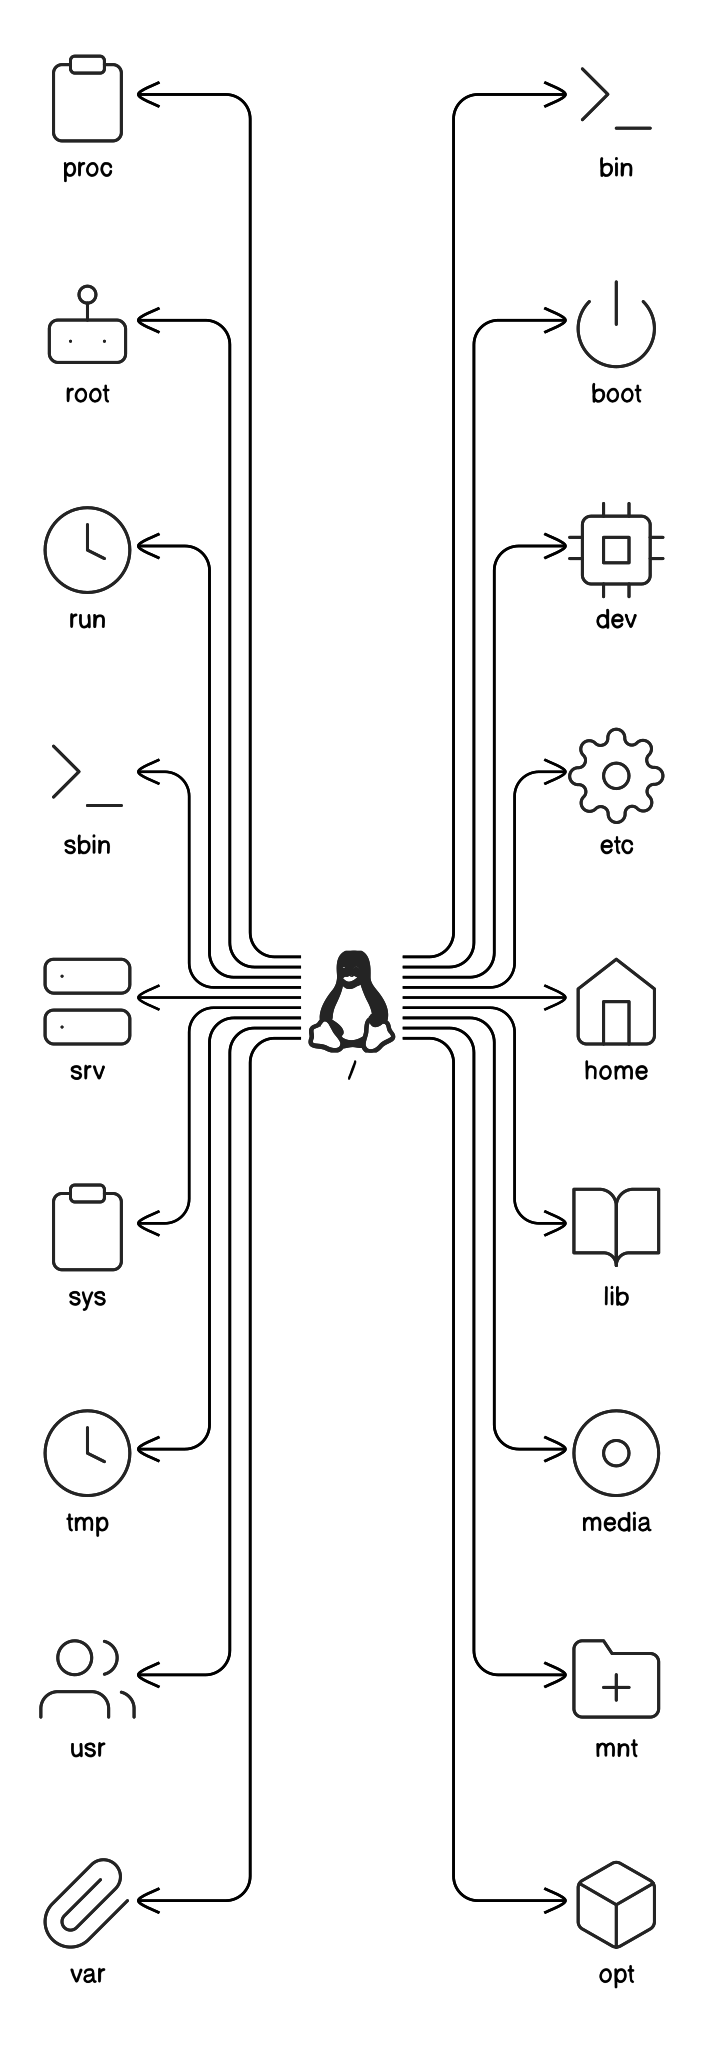
\includegraphics[width=0.7\linewidth]{linuxfs.pdf}
	\caption[Linux Filesystem Hierarchy]{Linux Filesystem Hierarchy}
	\labfig{linuxfs}
\end{figure}

Some directories do not store data on the disk, but are used to store information about the system.
These directories are called \textit{virtual} directories.
For example, the \textbf{/proc} directory is a virtual directory that provides information about the running processes.
The \textbf{/sys} directory is another virtual directory that provides information about the system.
The \textbf{/tmp} is a \textit{volatile} directory whose data is deleted as soon as the system is turned off.
The \textbf{/run} directory is another volatile directory that stores runtime data.

Rest directories are stored on the disk.
The reason for having so many directories is to categorize the type of files they store.
For example, all the executable binaries of different applications and utilities installed in the system is stored in \textbf{/bin} and \textbf{/sbin} directories.
All the shared libraries installed on the system are stored in \textbf{/lib} directory.
Sometimes some applications are installed in \textbf{/opt} directory which are not installed directly by the package manager.
\sidenote{
  In Linux, you do not install applications by downloading them from the internet and running an installer like in Windows. You use a package manager to install applications. The package manager downloads the application from the internet and installs it on your system automatically. This way the package manager can also keep track of the installed applications and their dependencies and whether they should be updated. This is similar to the \textit{Play Store} on mobile phones.
}

We also need to store the user's documents and files.
This is done in the \textbf{/home} directory.
Each user has their own directory in the \textbf{/home} directory.
The root user's directory is \textbf{/root}.
All the application's configuration files are stored in the user's home directory in the \textbf{/home} directory itself.
This separation of application binary and per-user application settings helps people to easily change systems but keep their own \textbf{/home} directory constant and in turn, also all their application settings.

Some settings however needs to be applied system-wide and for all users.
These settings are stored in the \textbf{/etc} directory.
This directory contains all the system-wide configuration files.

To boot up the system, the bootloader needs some files. These files are stored in the \textbf{/boot} directory.
\sidenote{
  Modern systems use \textbf{UEFI} instead of \textbf{BIOS} to boot up the system. The bootloader is stored in the \textbf{/boot/EFI} directory or in the \textbf{/efi} directory directly.
}
The bootloader is the first program that runs when the computer is turned on. It loads the operating system into memory and starts it.

Although the file system is a unified tree hierarchy, this doesn't mean that we cannot have multiple partitions on Linux: au contraire, it is easier to manage partitions on Unix.
We simply need to mention which empty directory in the hierarchy should be used to mount a partition.
As soon as that partition is mounted, it gets populated with the data stored on that disk with all the files and subdirectories, and when the device is unmounted the directory again becomes empty.
Although a partition can be mounted on any directory, there are some dedicated folders in \lstinline|/| as well for this purpose.
For example, the \lstinline|/mnt| directory is used to mount a filesystem temporarily, and the \lstinline|/media| directory is used to mount removable media like USB drives, however it is not required to strictly follow this.

Finally, the biggest revelation in Linux is that, everything is a file.
Not only are all the system configurations stored as \textbf{plain text} files which can be read by humans, but the processes running on your system are also stored as files in proc.
Your kernel's interfaces to the applications or users are also simple files stored in sys.
Biggest of all, even your hardware devices are stored as files in dev.
\sidenote{
  Device files are not stored as normal files on the disk, but are special files that the kernel uses to communicate with the hardware devices.
  These are either \textbf{block} or \textbf{character} devices.
  They are used to read and write data to and from the hardware devices.
}

The \textbf{/usr} directory is a secondary hierarchy that contains subdirectories similar to those present in \textbf{/}.
This was created as the olden system had started running out of disk space for the \textbf{/bin} and \textbf{/lib} directories.
Thus another directory named \textbf{usr} was made, and subdirectiores like \textbf{/usr/bin} and \textbf{/usr/lib} were made to store half of the binaries and libraries.
There wasn't however any rigid definition of which binary should go where.
Modern day systems have more than enough disk space to store everything on one partition, thus the \textbf{/bin} and \textbf{/lib} dont really exist any more. If they do, they are simply shortcuts
\sidenote{
  Shortcuts in Linux are called \textit{symbolic links} or \textit{symlinks}.
}
to the \textbf{/usr/bin} and \textbf{/usr/lib} directories which are still kept for \textit{backwards compatibility}.

These can also be loosely classified into \textit{sharable} and \textit{non-sharable} directories and \textit{static} and \textit{variable} directories as shown in \vreftab{linuxfsclass-table}.

\begin{table}[h!]
\caption{Linux Filesystem Directory Classification}
\labtab{linuxfsclass-table}
\begin{tabular}{ c | c c }
  \toprule
  & Sharable & Non-sharable \\
 \midrule
  Static & /usr, /opt & /etc, /boot \\
  Variable & /var/spool & /tmp, /var/log \\
 \bottomrule
\end{tabular}
\end{table}

\subsection{In Memory File System}

Some file systems like \textbf{proc}, \textbf{sys}, \textbf{dev}, \textbf{run}, and \textbf{tmp} are not stored on the disk, but are stored in memory.

They have a special purpose and are used to store information about the system.
These are called \textit{virtual} directories.

These cannot be stored in a disk as it would be too slow to access them.
Many of these files are very short lived yet are accessed very frequently.
So these are stored in memory to speed up the access.

\textbf{/dev} and \textbf{/run} are mounted as \textbf{tmpfs} filesystems.

This can be seen by running the \lstinline|mount| command or the \lstinline|df| command.

\begin{lstlisting}[language=bash]
  $ mount
/dev/sda1 on / type ext4 (rw,noatime)
devtmpfs on /dev type devtmpfs (rw,nosuid,size=4096k,nr_inodes=990693,mode=755,inode64)
tmpfs on /dev/shm type tmpfs (rw,nosuid,nodev,inode64)
devpts on /dev/pts type devpts (rw,nosuid,noexec,relatime,gid=5,mode=620,ptmxmode=000)
sysfs on /sys type sysfs (rw,nosuid,nodev,noexec,relatime)
securityfs on /sys/kernel/security type securityfs (rw,nosuid,nodev,noexec,relatime)
cgroup2 on /sys/fs/cgroup type cgroup2 (rw,nosuid,nodev,noexec,relatime,nsdelegate,memory_recursiveprot)
pstore on /sys/fs/pstore type pstore (rw,nosuid,nodev,noexec,relatime)
efivarfs on /sys/firmware/efi/efivars type efivarfs (rw,nosuid,nodev,noexec,relatime)
bpf on /sys/fs/bpf type bpf (rw,nosuid,nodev,noexec,relatime,mode=700)
configfs on /sys/kernel/config type configfs (rw,nosuid,nodev,noexec,relatime)
proc on /proc type proc (rw,nosuid,nodev,noexec,relatime)
tmpfs on /run type tmpfs (rw,nosuid,nodev,size=1590108k,nr_inodes=819200,mode=755,inode64)
systemd-1 on /proc/sys/fs/binfmt_misc type autofs (rw,relatime,fd=36,pgrp=1,timeout=0,minproto=5,maxproto=5,direct,pipe_ino=5327)
hugetlbfs on /dev/hugepages type hugetlbfs (rw,nosuid,nodev,relatime,pagesize=2M)
mqueue on /dev/mqueue type mqueue (rw,nosuid,nodev,noexec,relatime)
debugfs on /sys/kernel/debug type debugfs (rw,nosuid,nodev,noexec,relatime)
tracefs on /sys/kernel/tracing type tracefs (rw,nosuid,nodev,noexec,relatime)
fusectl on /sys/fs/fuse/connections type fusectl (rw,nosuid,nodev,noexec,relatime)
systemd-1 on /data type autofs (rw,relatime,fd=47,pgrp=1,timeout=60,minproto=5,maxproto=5,direct,pipe_ino=2930)
tmpfs on /tmp type tmpfs (rw,noatime,inode64)
/dev/sda4 on /efi type vfat (rw,relatime,fmask=0137,dmask=0027,codepage=437,iocharset=ascii,shortname=mixed,utf8,errors=remount-ro)
/dev/sda2 on /home type ext4 (rw,noatime)
binfmt_misc on /proc/sys/fs/binfmt_misc type binfmt_misc (rw,nosuid,nodev,noexec,relatime)
tmpfs on /run/user/1000 type tmpfs (rw,nosuid,nodev,relatime,size=795052k,nr_inodes=198763,mode=700,uid=1000,gid=1001,inode64)
portal on /run/user/1000/doc type fuse.portal (rw,nosuid,nodev,relatime,user_id=1000,group_id=1001)
/dev/sdb3 on /data type ext4 (rw,noatime,x-systemd.automount,x-systemd.idle-timeout=1min)
\end{lstlisting}

Here we can see that the \textbf{/dev} directory is mounted as a \textbf{devtmpfs} filesystem.
The \textbf{/run} directory is mounted as a \textbf{tmpfs} filesystem.
The \textbf{/proc} directory is mounted as a \textbf{proc} filesystem.
The \textbf{/sys} directory is mounted as a \textbf{sysfs} filesystem.

These are all virtual filesystems that are stored in memory.

\textbf{proc}:

Proc is an old filesystem that is used to store information about the running processes.
The \textbf{/proc} directory contains a directory for each running process.
The directories are named as the process id of the process.

\begin{lstlisting}[language=bash]
$ ls -l /proc | head
total 0
dr-xr-xr-x  9 root  root  0 May 23 13:01 1
dr-xr-xr-x  9 root  root  0 May 23 13:01 100
dr-xr-xr-x  9 sayan sayan 0 May 23 13:06 1004
dr-xr-xr-x  9 sayan sayan 0 May 23 13:06 1009
dr-xr-xr-x  9 root  root  0 May 23 13:01 102
dr-xr-xr-x  9 root  sayan 0 May 23 13:06 1029
dr-xr-xr-x  9 sayan sayan 0 May 23 13:06 1038
dr-xr-xr-x  9 sayan sayan 0 May 23 13:06 1039
dr-xr-xr-x  9 sayan sayan 0 May 23 13:06 1074
\end{lstlisting}

These folders are simply for information and do not store any data.
This is why they have a size of 0.
Each folder is owned by the user who started the process.

Inside each of these directories, there are files that contain information about the process.

You can enter the folder of a process that is started by you and see the information about the process.

\begin{lstlisting}[language=bash]
$ cd /proc/301408
$ ls -l | head -n15
total 0
-r--r--r--  1 sayan sayan 0 May 23 16:55 arch_status
dr-xr-xr-x  2 sayan sayan 0 May 23 16:55 attr
-rw-r--r--  1 sayan sayan 0 May 23 16:55 autogroup
-r--------  1 sayan sayan 0 May 23 16:55 auxv
-r--r--r--  1 sayan sayan 0 May 23 16:55 cgroup
--w-------  1 sayan sayan 0 May 23 16:55 clear_refs
-r--r--r--  1 sayan sayan 0 May 23 16:55 cmdline
-rw-r--r--  1 sayan sayan 0 May 23 16:55 comm
-rw-r--r--  1 sayan sayan 0 May 23 16:55 coredump_filter
-r--r--r--  1 sayan sayan 0 May 23 16:55 cpu_resctrl_groups
-r--r--r--  1 sayan sayan 0 May 23 16:55 cpuset
lrwxrwxrwx  1 sayan sayan 0 May 23 16:55 cwd -> /home/sayan/docs/projects/sc-handbook
-r--------  1 sayan sayan 0 May 23 16:55 environ
lrwxrwxrwx  1 sayan sayan 0 May 23 13:41 exe -> /usr/bin/entr
\end{lstlisting}

Here you can see that the command line of the process is stored in the \textbf{cmdline} file.
Here the process is of a command called \textbf{entr}.

You can also see the \textbf{current working directory} (cwd) of the process.

There are some other files in the \textbf{/proc} directory that contain information about the system.

\begin{itemize}
  \item \textbf{cpuinfo} - stores cpu information.
  \item \textbf{version} - stores system information, content similar to \lstinline|uname -a| command.
  \item \textbf{meminfo} - Diagnostic information about memory. Check \lstinline|free| command.
  \item \textbf{partitions} - Disk partition information. Check \lstinline|df|.
  \item \textbf{kcore} - The astronomical size ( $2^{47}$ bits) tells the maximum virtual memory (47 bits) the current Linux OS is going to handle.
\end{itemize}

\textbf{sys}:

Sys is a newer filesystem that is used to store information about the system.
It is neatly organized and is easier to navigate than proc.
This highly uses symlinks to organize the folders while maintaining redundancy as well.
\sidenote{
  A symlink is a special type of file that points to another file or directory.
  It is similar to a shortcut in Windows.
  This will be discussed in detail in \refsec{inodes-links}.
}

Try running the following code snippet in a terminal if you have a caps lock key on your keyboard and are running linux directly on your bare-metal.
\sidenote{
  This will only work on your own system, not on the system commands VM, since you do not have the priviledge to modify the files there.
  Make sure you have the ability to run commands as root and are able to use \lstinline|sudo|.
  It is also unlikely to work on a virtual machine.
  It will also not work on linux systems older than 2.6.
}

\begin{lstlisting}[language=bash]
  $ cd /sys/class/leds
  $ echo 1 | sudo tee *capslock/brightness
\end{lstlisting}

If you are running a linux system directly on your hardware, you will see the caps lock key light up.
Most modern keyboards will quickly turn off the light again as the capslock is technically not turned on, only the led was turned on manually by you.

\textbf{/sys vs /proc}:

The \lstinline|/proc| tree originated in System V Unix
\sidenote{
  Unix System V is one of the first commercial versions of the Unix operating system. It was originally developed by AT\&T and first released in 1983.
}
, where it only gave information about each running process, using a
\lstinline|/proc/\$PID/| format. Linux greatly extended that, adding all sorts of information about the running kernel's status. In addition to these read-only information files, Linux's \lstinline|/proc| also has writable virtual files that can change the state of the running kernel.
BSD
\sidenote{
  BSD, or Berkeley Software Distribution, is a Unix-like operating system that was developed at the University of California, Berkeley. It was first released in 1977 and was based on the original Unix source code from AT\&T. BSD is not linux, it is a totally different kernel, with similar core utils to GNU.
}
type OSes generally do not have \lstinline|/proc| at all, so much of what you find under proc is non-portable.

The intended solution for this mess in Linux's \lstinline|/proc| is \lstinline|/sys|. Ideally, all the non-process information that got crammed into the \lstinline|/proc| tree should have moved to \lstinline|/sys| by now, but historical inertia has kept a lot of stuff in \lstinline|/proc|.
Often there are two ways to effect a change in the running kernel: the old \lstinline|/proc| way, kept for backwards compatibility, and the new \lstinline|/sys| way that you're supposed to be using now.
% \sidecite{sysvproc}

\subsection{Paths}

Whenever we open a terminal on a Linux system, we are placed in a directory.
This is called the \textit{current working directory}.
All shells and applications have a current working directory from where they are launched.

To refer to and identify the directory you are talking about, we use a \textbf{path}.

\begin{definition}[Path]
  Path is a traversal in the filesystem tree.
  It is a way to refer to a file or directory.
\end{definition}

\textbf{Absolute Path:}

The traversal to the directory from the root directory is called the \textbf{absolute path}. For example, if we want to refer to the directory named \textbf{alex} inside the directory \textbf{home} in the root of the file system, then it is qualified as:

\begin{lstlisting}[language=bash]
  /home/alex
\end{lstlisting}

\textbf{Relative Path:}

\begin{marginfigure}
	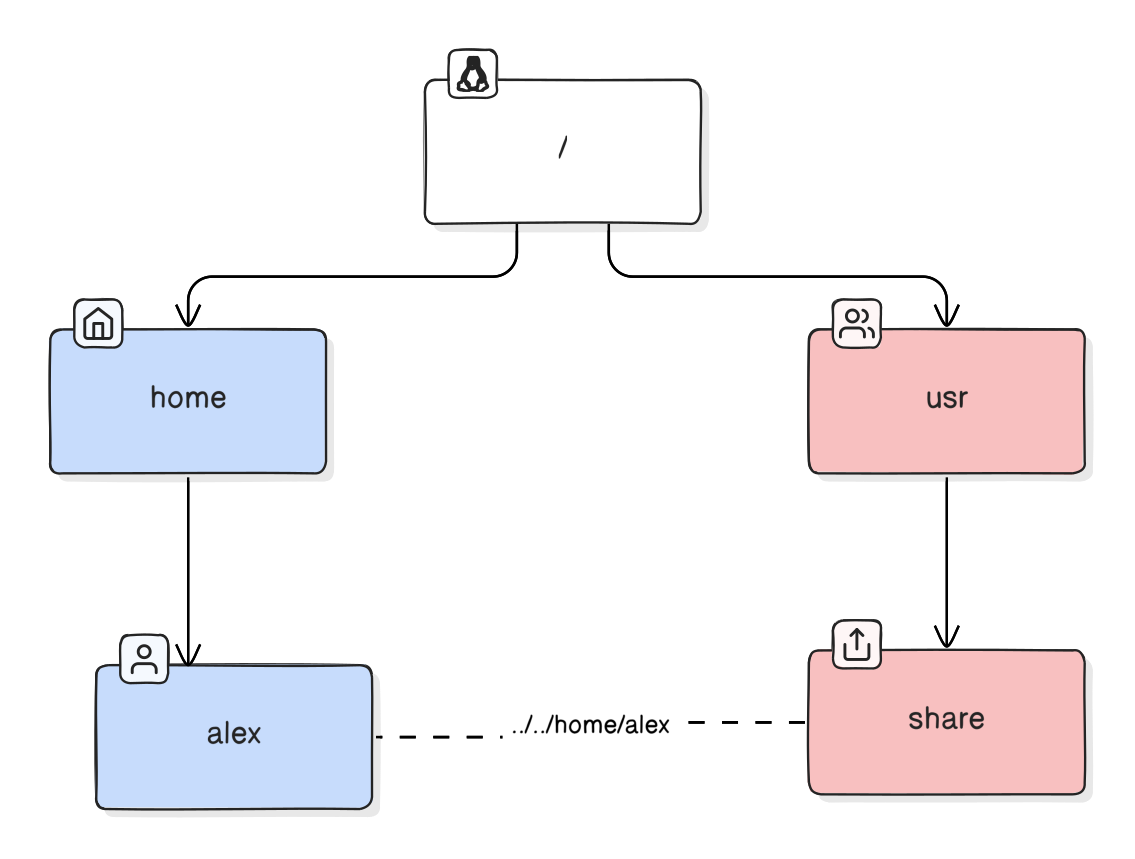
\includegraphics{relpath.pdf}
	\caption[Relative Path]{Relative Path}
	\labfig{relpath}
\end{marginfigure}

The traversal to the directory from the current working directory is called the \textbf{relative path}. For example, if we want to refer to the directory named \textbf{alex} inside the directory \textbf{home} from the \textbf{/usr/share} directory, then it will be qualified as:

\begin{lstlisting}[language=bash]
  ../../home/alex
\end{lstlisting}

\begin{remark}
  The \textbf{..} in the path refers to the parent directory. It is used in relative paths to refer to directories whose path requires travelling up the tree.
\end{remark}

\subsection{Basic Commands for Navigation}
The file system can be navigated in the Linux command line using the following commands:
\begin{itemize}
  \item \textbf{pwd}: Print the current working directory
  \item \textbf{ls}: List the contents of the current directory
  \item \textbf{cd}: Change the current working directory
  \item \textbf{mkdir}: Create a new directory
  \item \textbf{rmdir}: Remove a directory
  \item \textbf{touch}: Create a new file
  \item \textbf{rm}: Remove a file
  \item \textbf{pushd}: Push the current directory to a stack
  \item \textbf{popd}: Pop the current directory from a stack\sidenote{\textbf{pushd} and \textbf{popd} are useful for quickly switching between directories in scripts.}
\end{itemize}

More details about these commands can be found in their respective
man pages. For example, to find more about the \textbf{ls} command,
you can type \lstinline|man ls|.

\begin{qs}
  What is the command to list the contents of the current directory?
\end{qs}

\begin{ans}
  \lstinline|ls|
\end{ans}


\begin{qs}
  What is the command to list the contents of the current directory
  including hidden files?
\end{qs}

\begin{ans}
\lstinline|ls -a|
\end{ans}

\begin{qs}
  What is the command to list the contents of the current directory
  in a long list format? (show permissions, owner, group, size, and time)
\end{qs}

\begin{ans}
\lstinline|ls -l|
\end{ans}

\begin{qs}
  What is the command to list the contents of the current directory
  in a long list format and also show hidden files?
\end{qs}

\begin{ans}
\lstinline|ls -al| or \lstinline|ls -la| or \lstinline|ls -l -a| or \lstinline|ls -a -l|
\end{ans}

\begin{qs}
  The output of \lstinline|ls| gives multiple files and directories in a single
  line. How can you make it print one file or directory per line?
\end{qs}

\begin{ans}
  \lstinline|ls -1|\\
  This can also be done by passing the output of \lstinline|ls| to \lstinline|cat|
  or storing the output of \lstinline|ls| in a file and then using \lstinline|cat|
  to print it. We will see these in later weeks.\sidenote{that is a one, not an L}
\end{ans}

\vfill
\pagebreak
\section{File Permissions}
\labsec{file-permissions}

\begin{figure}[hb]
  \includegraphics{perms}
  \caption[File Permissions]{File Permissions}
  \labfig{perms}
\end{figure}

\begin{definition}[File Permissions]
  File permissions define the access rights of a file or directory.
  There are three basic permissions: read, write, and execute.
  These permissions can be set for the owner of the file, the group of the file, and others.
\end{definition}

We have already briefly seen how to see the permissions of a file using the \lstinline[language=bash]{ls -l} command.

\begin{lstlisting}[language=bash]
  $ touch hello.txt
  $ mkdir world
  $ ls -l
  total 4
  -rw-r--r-- 1 sayan sayan    0 May 21 15:20 hello.txt
  drwxr-xr-x 2 sayan sayan 4096 May 21 15:21 world
\end{lstlisting}

Here, the first column of the output of \lstinline|ls -l| shows the permissions of the file or directory.
As seen in \reffig{perms}, the permissions are divided into four parts:

\begin{itemize}
  \item The first character shows the type of the file. \lstinline|-| for a regular file and \lstinline|d| for a directory and more.
    \sidenote{
      There are other types of files as well, like \lstinline|l| for a symbolic link, \lstinline|c| for a character device, \lstinline|b| for a block device, \lstinline|s| for a socket, and \lstinline|p| for a pipe. These will be discussed later.
    }
  \item The next three characters show the permissions for the owner of the file.
  \item The next three characters show the permissions for the group of the file.
  \item The last three characters show the permissions for others.
\end{itemize}

\begin{definition}[Owner]
  Although this can be changed, the owner of a file is usually the user who created it.
  All files in the filesystem have an owner.
  This is symbolically coded as \textbf{u}.
\end{definition}

\begin{definition}[Group]
  The group of a file is usually the group of the user who created it.
  But it can also be changed to any other existing group in the system.
  All users in the group
  \footnote{
    except the owner of the file
  }
  have the same permissions on the file.
  This is symbolically coded as \textbf{g}.
\end{definition}

\begin{definition}[Others]
  Others are all the users who are not the owner of the file and are not in the group of the file.
  This is symbolically coded as \textbf{o}.
\end{definition}

There are three actions that can be performed on a file: read, write, and execute.

\begin{itemize}
  \item \textbf{Read}: The read permission allows the file to be read.
    This is symbolically coded as \textbf{r}.
  \item \textbf{Write}: The write permission allows the file to be modified.
    This is symbolically coded as \textbf{w}.
  \item \textbf{Execute}: The execute permission allows the file to be executed.
    \sidenote{
      Executing a file means running the file as a program.
      For a directory, the execute permission allows the directory to be traversed into.
    }
    This is symbolically coded as \textbf{x}.
\end{itemize}

These however, have different meanings for files and directories.

\subsection{Read}

\begin{itemize}
  \item For a file, the read permission allows the file to be read.
    You can use commands like \lstinline|cat| or \lstinline|less| to read the contents of the file if the user has \textbf{read} permissions.
  \item For a directory, the read permission allows the directory to be listed using \lstinline|ls|.
\end{itemize}

\subsection{Write}

\begin{itemize}
  \item For a file, the write permission allows the file to be modified.
    You can use commands like \lstinline|echo| along with redirection
    \sidenote{
      Redirection is a way to send the output of a command to a file.
    }
    or a text editor like \lstinline|vim| or \lstinline|nano|
      to write to the file if the user has \textbf{write} permissions.
  \item For a directory, the write permission allows the directory to be modified.
    You can create, delete, or rename files in the directory if the user has \textbf{write} permissions.
\end{itemize}

\subsection{Execute}

\begin{itemize}
  \item For a file, the execute permission allows the file to be executed.
    This is usually only needed for special files like executables,
    scripts, or libraries.
    You can run the file as a program if the user has \textbf{execute} permissions.
  \item For a directory, the execute permission allows the directory to be traversed into.
    You can change to the directory if the user has \textbf{execute} permissions using \lstinline|cd|.
    You can also only long-list the contents of the directory if the user has \textbf{execute} permissions on that directory.
\end{itemize}

\subsection{Interesting Caveats}

This causes some interesting edge-cases that one needs to be familiar with.

\textbf{Cannot modify a file? Think again!}

If you have \textbf{write} and \textbf{execute} permissions on a directory, even if you do not have \textbf{write} permission on a file inside the directory, you can \textbf{delete} the file due to your \textbf{write} permission on the directory, and then re-create the modified version of the file with the same name.
But if you try to simply modify the file directly, you will get permission error.

\begin{lstlisting}[language=bash]
  $ mkdir test
  $ cd test
  $ echo "hello world" > file1
  $ chmod 400 file1     # 400 means read permission only
  $ cat file1
  hello world
  $ echo "hello universe" > file1  # unable to write
  -bash: file1: Permission denied
  $ rm file1  # can remove as we have write permission on folder
  rm: remove write-protected regular file 'file1'? y
  $ echo "hello universe" > file1 # can create new file
  $ cat file1
  hello universe
\end{lstlisting}

However, this only works on files.
You cannot remove a directory if you do not have \textbf{write} permission on the directory, even if you have \textbf{write} permission on its parent directory.

\textbf{Can list names but not metadata?}

If you have \textbf{read} permission on a directory but not \textbf{execute} permission, you cannot traverse into the directory, but you can still use \lstinline|ls| to list the contents of the directory.
However, you cannot use \lstinline|ls -l| to long-list the contents of the directory.
That is, you only have access to the name of the files inside, not their metadata.

\begin{lstlisting}[language=bash]
  $ mkdir test
  $ touch test/1 test/2
  $ chmod 600 test # removing execute permission from folder
  $ ls test # we can still list the files due to read permission
  1  2
  $ ls -l test # but cannot long-list the files
  ls: cannot access 'test/2': Permission denied
  ls: cannot access 'test/1': Permission denied
  total 0
  -????????? ? ? ? ?            ? 1
  -????????? ? ? ? ?            ? 2
\end{lstlisting}

\textbf{Cannot list names but can traverse?}

If you have \textbf{execute} permission on a directory but not \textbf{read} permission, you can traverse into the directory but you cannot list the contents of the directory.

\begin{lstlisting}[language=bash]
  $ mkdir test
  $ touch test/1 test/2
  $ chmod 300 test # removing read permission from folder
  $ ls test # we cannot list the files
  ls: cannot open directory 'test': Permission denied
  $ cd test # but we can traverse into the folder
  $ pwd
  /home/sayan/test
\end{lstlisting}

\textbf{Subdirectories with all permissions, still cannot access?}

If you have all the permissions to a directory, but dont have
\textbf{execute} permission on its parent directory,
you cannot access the subdirectory, or even list its contents.

\begin{lstlisting}[language=bash]
  $ mkdir test
  $ mkdir test/test2 # subdirectory
  $ touch test/test2/1 # file inside subdirectory
  $ chmod 700 test/test2 # all permissions to subdirectory
  $ chmod 600 test # removing execute permission from parent directory
  $ ls test
  test2
  $ cd test/test2 # cannot access subdirectory
  -bash: cd: test/test2: Permission denied
  $ ls test/test2 # cannot even list contents of subdirectory
  ls: cannot access 'test/test2': Permission denied
\end{lstlisting}

\subsection{Changing Permissions}

The permissions of a file can be changed using the \textbf{chmod} command.

\textbf{Synopsis:}

\begin{lstlisting}[language=bash]
  chmod [OPTION]... MODE[,MODE]... FILE...
  chmod [OPTION]... OCTAL-MODE FILE...
\end{lstlisting}

\textbf{OCTAL-MODE} is a 3 or 4 digit octal number where the first digit is for the owner, the second digit is for the group, and the third digit is for others.
We will discuss how the octal representation of permissions is calculated in the next section.

The \textbf{MODE} can be in the form of \textbf{ugoa+-=rwxXst} where:

\begin{itemize}
  \item \textbf{u} is the user who owns the file
  \item \textbf{g} is the group of the file
  \item \textbf{o} is others
  \item \textbf{a} is all
  \item \textbf{+} adds the permission
  \item \textbf{-} removes the permission
  \item \textbf{={}} sets the permission
  \item \textbf{r} is read
  \item \textbf{w} is write
  \item \textbf{x} is execute
  \item \textbf{X} is execute only if its a directory or already has execute permission.
  \item \textbf{s} is setuid/setgid
  \item \textbf{t} is restricted deletion flag or sticky bit
\end{itemize}

We are already familiar with what
\textbf{r},
\textbf{w}, and
\textbf{x}
permissions mean, but what are the other permissions?

\subsection{Special Permissions}
\labsec{special-permissions}

\begin{definition}[SetUID/SetGID]
  The setuid and setgid bits are special permissions that can be set on executable files.
  When an executable file has the setuid bit set, the file will be executed with the privileges of the owner of the file.
  When an executable file has the setgid bit set, the file will be executed with the privileges of the group of the files.
\end{definition}

\textbf{SetUID}:

This is useful for programs that need to access system resources that are only available to the owner or group of the file.

A very notable example is the \lstinline|passwd| command.
This command is used to set the password of an user.
Although changing password of a user is a priviledged action that only the root user can do, the \lstinline|passwd| command can be run by any user to change \textit{their} password.
This is possible due to the setuid bit set on the \lstinline|passwd| command.
When the \lstinline|passwd| command is run, it is run with the privileges of the root user, and thus can change the password of that user.

You can check this out by running \lstinline|ls -l /usr/bin/passwd| and seeing the \lstinline|s| in the permissions.

\begin{lstlisting}[language=bash]
  $ ls -l /usr/bin/passwd
  -rwsr-xr-x 1 root root 80912 Apr  1 15:49 /usr/bin/passwd
\end{lstlisting}

\textbf{SetGID}:

The behaviour of \textbf{SetGID} is similar to \textbf{SetUID}, but the file is executed with the privileges of the group of the file.

However, \textbf{SetGID} can also be applied to a directory.
When a directory has the \textbf{SetGID} bit set, all the files and directories created inside that directory will inherit the group of the directory, not the group of the user who created the file or directory.
This is highly useful when you have a directory where multiple users need to work on the same files and directories, but you want to restrict the access to only a certain group of users.
The primary group of each user is different from each other, but since they are also part of another group (which is the group owner of the directory) they are able to read and write the files present in the directory.
However, if the user creates a file in the directory, the file will be owned by the user's primary group, not the group of the directory.
So other users would not be able to access the file.
This is fixed by the \textbf{SetGID} bit on the directory.

\begin{lstlisting}[language=bash]
  $ mkdir test
  $ ls -ld test # initially the folder is owned by the user's primary group
  drwxr-xr-x 2 sayan sayan 4096 May 22 16:27 test
  $ chgrp wheel test # we change the group of the folder to wheel, which is a group that the user is part of
  $ ls -ld test
  drwxr-xr-x 2 sayan wheel 4096 May 22 16:27 test
  $ whoami # this is the current user
  sayan
  $ groups # this is the users groups, first one is its primary group
  sayan wheel
  $ touch test/file1 # before setting the SetGID bit, a new file will have group owner as the primary group of the user creating it
  $ ls -l test/file1 # notice the group owner is sayan
  -rw-r--r-- 1 sayan sayan 0 May 22 16:29 test/file1
  $ chmod g+s test # we set the SetGID bit on the directory
  $ ls -ld test # now the folder has a s in the group permissions
  drwxr-sr-x 2 sayan wheel 4096 May 22 16:29 test
  $ touch test/file2 # now if we create another new file, it will have the group owner as the group of the directory
  $ ls -l test/file2 # notice the group owner is wheel
  -rw-r--r-- 1 sayan wheel 0 May 22 16:29 test/file2
\end{lstlisting}

\textbf{Restricted Deletion Flag or Sticky Bit}:

The restricted deletion flag or sticky bit is a special permission that can be set on directories.

Historically, this bit was to be applied on executable files to keep the program in memory after it has finished executing.
This was done to speed up the execution of the program as the program would not have to be loaded into memory again.
This was called \textbf{sticky bit} because the program would stick in memory.
\sidenote{
  The part of memory where the program's text segment is stored is called the \textit{swap}.
}

However, this is no longer how this bit is used.

When the sticky bit is set on a directory, only the owner of the file, the owner of the directory, or the root user can delete or rename files in the directory.

This is useful when you have a directory where multiple users need to write files, but you want to restrict the deletion of files to only the owner of the file or the owner of the directory.

The most common example of this is the \lstinline|/tmp| directory.
The \lstinline|/tmp| directory is a directory where temporary files are stored.
You want to let any user create files in the \lstinline|/tmp| directory, but you do not want any user to delete files created by other users.

\begin{lstlisting}[language=bash]
  $ ls -ld /tmp
  drwxrwxrwt 20 root root 600 May 22 16:43 /tmp
\end{lstlisting}

\begin{exercise}
  Log into the system commands VM and cd into the \lstinline|/tmp| directory.
  Create a file in the \lstinline|/tmp| directory.
  Try to find if there are files created by other users in the \lstinline|/tmp| directory using \lstinline|ls -l| command.
  If there are files created by other users, try to delete them.
  \footnote{
    You can create a file normally, or using the \textbf{mktemp} command.
  }
\end{exercise}

\subsection{Octal Representation of Permissions}

\begin{figure}
  \includegraphics{octal-permissions}
  \caption[Octal Permissions]{Octal Permissions}
  \labfig{octal-permissions}
\end{figure}

The permissions of a file for the file's owner, group, and others can be represented as a 3 or 4 digit octal number.
\sidenote{
  If the octal is 4 digits, the first digit is for special permissions like setuid, setgid, and sticky bit.
}
Each of the octal digits is the sum of the permissions for the owner, group, and others.

\begin{itemize}
  \item \textbf{Read} permission is represented by 4
  \item \textbf{Write} permission is represented by 2
  \item \textbf{Execute} permission is represented by 1
\end{itemize}

Thus if a file has read, write, and execute permissions for the owner, read and execute permissions for the group, and only read permission for others, the octal representation of the permissions would be 754.

\begin{table*}
\caption{Octal Representation of Permissions}
\labtab{octal-permissions-table}
\begin{tabular}{ c c c c c c }
  \toprule
  Octal & Read & Write & Execute & Representation & Description \\
 \midrule
  0 & 0 & 0 & 0 & --- & No permissions \\
  1 & 0 & 0 & 1 & --x & Execute only \\
  2 & 0 & 1 & 0 & -w- & Write only \\
  3 & 0 & 1 & 1 & -wx & Write and execute \\
  4 & 1 & 0 & 0 & r-- & Read only \\
  5 & 1 & 0 & 1 & r-x & Read and execute \\
  6 & 1 & 1 & 0 & rw- & Read and write \\
  7 & 1 & 1 & 1 & rwx & Read, write, and execute \\
 \bottomrule
\end{tabular}
\end{table*}

The octal format is usually used more than the symbolic format as it is easier to understand and remember and it is more concise.

\begin{lstlisting}
$ chmod 754 myscript.sh # this sets the permissions of myscript.sh to rwxr-xr--
$ ./myscript.sh
Hello World!
\end{lstlisting}

However, if you want to add or remove a permission without changing the other permissions, the symbolic format is more useful.

\begin{lstlisting}
$ chmod u+x myscript.sh # this adds execute permission to the owner of myscript.sh
$ ./myscript.sh
Hello World!
\end{lstlisting}

\begin{qs}
  How to list the permissions of a file?
\end{qs}

\begin{ans}
  \lstinline|ls -l| \\
  The permissions are the first 10 characters of the output.\\
  \lstinline|stat -c \%A filename| will list only the permissions of a file.\\
  There are other format specifiers of \lstinline|stat| to show different statistics
  which can be found in \lstinline|man stat|.
\end{ans}

\begin{qs}
  How to change permissions of a file?
  Let's say we want to change \lstinline|file1|'s permissions to \lstinline|rwxr-xr--|
  What is the octal form of that?
\end{qs}

\begin{ans}
  \lstinline|chmod u=rwx,g=rx,o=r file1| will change the permissions of \lstinline|file1|\\
  The octal form of \lstinline|rwxr-xr--| is 754.\\
  So we can also use \lstinline|chmod 754 file1|\\
  Providing the octal is same as using \lstinline|=| to set the permissions.\\
  We can also use \lstinline|+| to add permissions and \lstinline|-| to remove permissions.
\end{ans}

% ----------------------------

\vfill
\pagebreak
\section{Types of Files}

We had briefly seen that the output of \lstinline|ls -l| shows the type of the file as the first character of the permissions.

There are 7 types of files in a linux file system as shown in \vreftab{file-types-table}.

\begin{margintable}
\caption{Types of Files}
\labtab{file-types-table}
\begin{tabular}{ c c }
  \toprule
  Type & Symbol \\
 \midrule
  Regular Files & -{} \\
  Directories & d \\
  Symbolic Links & l \\
  Character Devices & c \\
  Block Devices & b \\
  Named Pipes & p \\
  Sockets & s \\
 \bottomrule
\end{tabular}
\end{margintable}

\subsection{Regular Files}

Regular files are the most common type of file.
Almost all files are regular files.
Scripts and executable binaries are also regular files.
All the configuration files of the system are regular files as well.
The regular files are actually the only files that contain data and are stored on the disk.

\subsection{Directories}

Directories are files that contain a list of other files.
Directories do not contain data, they contain references to other files.
Usually the size of a directory is equal to the block size of the filesystem.
Directories have some special permissions that are different from regular files as discussed in \refsec{file-permissions}.

\subsection{Symbolic Links}

Symbolic links are files that point to other files.
They only consume the space of the path they are pointing to.
Symlinks
\sidenote{
  Symlinks is short for symbolic links.
}
are useful to create shortcuts to files or directories.
They are dependent on the original file and will stop working if the original file is deleted or moved.
They are discussed in detail in \refsec{inodes-links}.

\marginnote{
  There are another type of links called \textbf{hard links}.
  However, hard links are not files, they are pointers to the same inode.
  They do not consume extra space, and are not dependent on the original file.
  Hard links do not have a separate type, they are just regular files.
}

\subsection{Character Devices}

Character devices are files that represent devices that are accessed as a stream of bytes.
For example the keyboard, mouse, webcams, and most USB devices are character devices.
These are not real files stored on the disk, but are files that represent devices.
They can interacted with like a file using the \lstinline|read| and \lstinline|write| system calls to interact with the hardware directly.
These files are made available by the kernel and are stored in the \lstinline|/dev| directory.
Any read/write operation on a character device is monitored by the kernel and the data is sent to the device.

\begin{lstlisting}
$ cd /dev/input
$ ls -l
total 0
drwxr-xr-x 2 root root     220 May 22 13:49 by-id
drwxr-xr-x 2 root root     420 May 22 13:49 by-path
crw-rw---- 1 root input 13, 64 May 22 13:49 event0
crw-rw---- 1 root input 13, 65 May 22 13:49 event1
crw-rw---- 1 root input 13, 74 May 22 13:49 event10
crw-rw---- 1 root input 13, 75 May 22 13:49 event11
crw-rw---- 1 root input 13, 76 May 22 13:49 event12
crw-rw---- 1 root input 13, 77 May 22 13:49 event13
crw-rw---- 1 root input 13, 78 May 22 13:49 event14
crw-rw---- 1 root input 13, 79 May 22 13:49 event15
crw-rw---- 1 root input 13, 80 May 22 13:49 event16
crw-rw---- 1 root input 13, 81 May 22 13:49 event17
crw-rw---- 1 root input 13, 82 May 22 13:49 event18
crw-rw---- 1 root input 13, 83 May 22 13:49 event19
crw-rw---- 1 root input 13, 66 May 22 13:49 event2
crw-rw---- 1 root input 13, 84 May 22 13:49 event20
crw-rw---- 1 root input 13, 67 May 22 13:49 event3
crw-rw---- 1 root input 13, 68 May 22 13:49 event4
crw-rw---- 1 root input 13, 69 May 22 13:49 event5
crw-rw---- 1 root input 13, 70 May 22 13:49 event6
crw-rw---- 1 root input 13, 71 May 22 13:49 event7
crw-rw---- 1 root input 13, 72 May 22 13:49 event8
crw-rw---- 1 root input 13, 73 May 22 13:49 event9
crw-rw---- 1 root input 13, 63 May 22 13:49 mice
crw-rw---- 1 root input 13, 32 May 22 13:49 mouse0
crw-rw---- 1 root input 13, 33 May 22 13:49 mouse1
\end{lstlisting}

Here the \lstinline|event| and \lstinline|mouse| files are character devices that represent input devices like the keyboard and mouse.
Note the \textbf{c} in the permissions, which indicates that these are character devices.

\subsection{Block Devices}

Block devices are files that represent devices that are accessed as a block of data.
For example hard drives, SSDs, and USB drives are block devices.
These files also do not store actual data on the disk, but represent devices.
Any block file can be mounted as a filesystem.
We can interact with block devices using the \lstinline|read| and \lstinline|write| system calls to interact with the hardware directly.
For example, the \lstinline|/dev/sda| file represents the first hard drive in the system.

This makes it easy to write an image to a disk directly using the \lstinline|dd| command.
\sidenote{
  The \lstinline|dd| command is a powerful tool that can be used to copy and convert files.
  It is acronym of \textit{data duplicator}.
  However, it is also known as the \textit{disk destroyer} command, as it can be used to overwrite the entire disk if you are not careful with which disk you are writing the image to.
}

The following example shows how we can use the \lstinline|dd| command to write an image
\sidenote{
  ISO file
}
to a USB drive.
It is this easy to create a bootable USB drive for linux.

\begin{lstlisting}[language=bash]
  $ dd if=~/Downloads/archlinux.iso of=/dev/sdb bs=4M status=progress
\end{lstlisting}

Here \lstinline|if| is the input file, \lstinline|of| is the output file, \lstinline|bs| is the block size, and \lstinline|status| is to show the progress of the operation.

\begin{warn}
  Be very careful when using the \lstinline|dd| command.
  Make sure you are writing to the correct disk.
  Writing to the wrong disk can cause data loss.
\end{warn}


\subsection{Named Pipes}

Named pipes
\sidenote{
  Also known as FIFOs
}
are files that are used for inter-process communication.
They do not store the data that you write to them, but instead pass the data to another process.
A process can only write data to a named pipe if another process is reading from the named pipe.
\sidenote{
  and vice versa
}

\begin{lstlisting}
$ mkfifo pipe1
$ ls -l pipe1
prw-r--r-- -1 sayan sayan 0 May 22 18:22 pipe1
\end{lstlisting}

Here the \lstinline|p| in the permissions indicates that this is a named pipe.
If you now try to write to the named pipe, the command will hang until another process reads from the named pipe.
Try the following in two different terminals:

\textbf{Terminal 1}:
\begin{lstlisting}
$ echo "hello" > pipe1
\end{lstlisting}

\textbf{Terminal 2}:
\begin{lstlisting}
$ cat pipe1
\end{lstlisting}

You will notice that whichever command you run first will hang until the other command is run.

\subsection{Sockets}

Sockets are a special file type, similar to TCP/IP sockets, providing inter-process networking protected by the file system's access control.

This is similar to named pipes, but the difference is that named pipes are meant for IPC between processes in the same machine, whereas sockets can be used for communication across machines.

Try out the following in two different terminals:

\textbf{Terminal 1}:
\begin{lstlisting}
$ nc -lU socket.sock
\end{lstlisting}

\textbf{Terminal 2}:
\begin{lstlisting}
$ echo "hello" | nc -U socket.sock
\end{lstlisting}

Notice here, that if you run the command in terminal 2 first, it will error out with the text:
\begin{lstlisting}
nc: socket.sock: Connection refused
\end{lstlisting}

Only if we run them in correct order can you see the message "hello" being printed in terminal 1.
\sidenote{
  The \lstinline|nc| command is the netcat command.
  It is a powerful tool for network debugging and exploration.
  It can be used to create sockets, listen on ports, and send and receive data over the network.
  This will be discussed in more detail in the networking section and in the
  \textbf{Modern Application Development} course.
}

You can press \lstinline|Ctrl+C| to stop the \lstinline|nc| command in both terminals.

\subsection{Types of Regular Files}

Regular files can be further classified into different types based on the data they contain.
In Linux systems, the type of a file is determined by its \textbf{
  \href{https://developer.mozilla.org/en-US/docs/Web/HTTP/Basics_of_HTTP/MIME_types}{MIME}
} type.
The extension of a file does not determine its type, the contents of the file do.
It is thus common to have files without extensions in Linux systems, as they provide no value.

\marginnote{
  The bytes at the start of a file used to identify the type of file are called the \textbf{magic bytes}. \\
  More details can be found at:
  \url{https://en.wikipedia.org/wiki/List_of_file_signatures}
}

The \lstinline|file| command can be used to determine the type of a file.

\begin{lstlisting}[language=bash]
$ file /etc/passwd
/etc/passwd: ASCII text
$ file /bin/bash
/bin/bash: ELF 64-bit LSB pie executable, x86-64, version 1 (SYSV), dynamically linked, interpreter /lib64/ld-linux-x86-64.so.2, BuildID[sha1]=165d3a5ffe12a4f1a9b71c84f48d94d5e714d3db, for GNU/Linux 4.4.0, stripped
\end{lstlisting}

\begin{qs}
  What types of files are possible in a linux file system?
\end{qs}

\begin{ans}
  There are 7 types of files in a linux file system:
  \begin{itemize}
    \item Regular Files (starts with \lstinline|-|)
    \item Directories (starts with \lstinline|d|)
    \item Symbolic Links (starts with \lstinline|l|)
    \item Character Devices (starts with \lstinline|c|)
    \item Block Devices (starts with \lstinline|b|)
    \item Named Pipes (starts with \lstinline|p|)
    \item Sockets (starts with \lstinline|s|)
  \end{itemize}
\end{ans}

\begin{qs}
  How to know what kind of file a file is? Can we determine using
  its extension? Can we determine using its contents? What does
  \textit{MIME} mean?
How to get that?
\end{qs}

\begin{ans}
  The \lstinline|file| command can be used to determine the type of a file. \\
  The extension of a file does not determine its type. \\
  The contents of a file can be used to determine its type. \\
  MIME stands for Multipurpose Internet Mail Extensions. \\
  It is a standard that indicates the nature and format of a document. \\
  \lstinline|file -i filename| will give the MIME type of \lstinline|filename|.
\end{ans}

% ----------------------------

\vfill
\pagebreak
\section{Inodes and Links}
\labsec{inodes-links}

\subsection{Inodes}

\begin{definition}[Inodes]
  An inode is an index node.
  It serves as a unique identifier for a specific piece of metadata on a given filesystem.
\end{definition}

Whenever you run \lstinline|ls -l| and see all the details of a file, you are seeing the metadata of the file.
These metadata, however, are not stored in the file itself.
These data about the files are stored in a special data structure called an \textbf{inode}.

Each inode is stored in a common table and each filesystem mounted to your computer has its own inodes.
An inode number may be used more than once but never by the same filesystem.
The filesystem id combines with the inode number to create a unique identification label.

You can check how many inodes are used in a filesystem using the \lstinline|df -i| command.

\begin{lstlisting}
$ df -i
Filesystem       Inodes   IUsed    IFree IUse% Mounted on
/dev/sda1       6397952  909213  5488739   15% /
/dev/sda4             0       0        0     - /efi
/dev/sda2      21569536 2129841 19439695   10% /home
/dev/sdb3      32776192    2380 32773812    1% /data
$ df
Filesystem     1K-blocks      Used Available Use% Mounted on
/dev/sda1      100063312  63760072  31174076  68% /
/dev/sda4        1021952    235760    786192  24% /efi
/dev/sda2      338553420 273477568  47805068  86% /home
/dev/sdb3      514944248 444194244  44518760  91% /data
\end{lstlisting}

You can notice the number of inodes present, number of inodes used, and number of inodes that are free.
The \textbf{IUse\%} column shows the percentage of inodes used.
This however, does not mean how much of space is used, but how many files can be created.

Observe that although the \lstinline|/data| partition has only $1\%$ of inodes used, it has $91\%$ of space used.
This is because the files in the \lstinline|/data| partition are large files, and thus the number of inodes used is less.
Remember that a file will take up one inode, no matter how large it is.
But the space it takes up will be the size of the file.

We can also see the inode number of a file using the \lstinline|ls -i| command.

\begin{lstlisting}[language=bash]
$ ls -i
  1234567 file1
  1234568 file2
  1234569 file3
\end{lstlisting}

Here the first column is the \textbf{inode} number of the file.

\begin{remark}
  The inode number is unique only within the filesystem.
  If you copy a file from one filesystem to another, the inode number will change.
\end{remark}

\subsection{Separation of Data, Metadata, and Filename}

In UNIX systems, the data of a file and the metadata of a file are stored separately.
The inodes are stored in a inode-array or table, and contain the metadata of the file and the pointer to it in the storage block.
These metadata can be retrieved using the \lstinline|stat| system call.
\sidenote{
  A system call is a request in a operating system made via a software interrupt by an active process for a service performed by the kernel.
  The diagram in \reffig{system-calls} shows how system calls work.
}

\begin{marginfigure}
  \includegraphics{syscall}
  \caption[System Calls]{System Calls}
  \labfig{system-calls}
\end{marginfigure}

Conveniently, a userland utility to list the metadata of a file is also called \lstinline|stat|.

\begin{lstlisting}[language=bash]
$ stat /etc/profile
  File: /etc/profile
  Size: 993       	Blocks: 8          IO Block: 4096   regular file
Device: 8,1	Inode: 2622512     Links: 1
Access: (0644/-rw-r--r--)  Uid: (    0/    root)   Gid: (    0/    root)
Access: 2024-05-21 18:30:27.000000000 +0530
Modify: 2024-04-07 23:32:30.000000000 +0530
Change: 2024-05-21 18:30:27.047718323 +0530
 Birth: 2024-05-21 18:30:27.047718323 +0530
\end{lstlisting}

We can also specify the format of the output of the \lstinline|stat| command using the \lstinline|--format| or \lstinline|-c| flag to print only the metadata we want.

The data of the file is stored in the storage block.
The inode number indexes a table of inodes on the file system.
From the inode number, the kernel's file system driver can access the inode contents, including the location of the file, thereby allowing access to the file.

On many older file systems, inodes are stored in one or more fixed-size areas that are set up at file system creation time, so the maximum number of inodes is fixed at file system creation, limiting the maximum number of files the file system can hold.

Some Unix-style file systems such as JFS, XFS, ZFS, OpenZFS, ReiserFS, btrfs, and APFS omit a fixed-size inode table, but must store equivalent data in order to provide equivalent capabilities. Common alternatives to the fixed-size table include B-trees and the derived B+ trees.

\begin{remark}
  Although the inodes store the metadata of the file, the filename is not stored in the inode.
  It is stored in the directory entry.
  Thus the filename, file metdata, and file data are stored separately.
\end{remark}

\begin{table}
\caption{Metadata of a File}
\labtab{metadata-file}
\begin{tabular}{ c c }
  \toprule
  Metadata & Description \\
 \midrule
  Size & Size of the file in bytes \\
  Blocks & Number of blocks used by the file \\
  IO Block & Block size of the file system \\
  Device & Device ID of the file system \\
  Inode & Inode number of the file \\
  Links & Number of hard links to the file \\
  Access & Access time of the file (\lstinline|atime|) \\
  Modify & Modification time of the file (\lstinline|mtime|) \\
  Change & Change time of the inode (\lstinline|ctime|) \\
  Birth & Creation time of the file \\
 \bottomrule
 \end{tabular}
\end{table}


\subsection{Directory Entries}

\begin{figure*}[ht]
  \includegraphics{inodes}
  \caption[Inode and Directory Entry]{Inodes and Directory Entry}
  \labfig{inode-directory}
\end{figure*}

Unix directories are lists of association structures, each of which contains one filename and one inode number.
The file system driver must search a directory for a particular filename and then convert the filename to the correct corresponding inode number.

Thus to read a file from a directory, first the directory's directory entry is read which stores the name of the file and its inode number.
The kernel then follows the inode number to find the inode of the file.
The inode stores all the metadata of the file, and the location of the data of the file.
The kernel then follows the inode to find the data of the file.
This is shown in \reffig{inode-directory}.

So what happens if two directory entries point to the same inode?
This is called a \textbf{hard link}.

\subsection{Hard Links}

If multiple entries of the directory entry points to the same inode, they are called hard links.
Hard links can have different names, but they are the same file.
As they point to the same inode, they also have the same metadata.

This is useful if you want to have the same file in multiple directories without taking up more space.
It is also useful if you want to keep a backup of a important file which is accessed by many people.
If someone accidentally deletes the file, the other hard links will still be there and able to access the file.

\begin{definition}[Hard Links]
  Hard Links are just pointers to the same inode. They are the same file.
  They are not pointers to the path of the file. They are pointers to the
  file itself. They are not affected by the deletion of the other file.
  When creating a hard link, you need to provide the path of the original
  file, and thus it has to be either absolute path, or relative from the
  current working directory, not relative from the location of the hard link.
\end{definition}

Hard links can be created for files only, and not directories.
It can be created using the \lstinline|ln| command.

\begin{lstlisting}[language=bash]
$ ln file1 file2
\end{lstlisting}

This will create a hard link named \lstinline|file2| that points to the same inode as \lstinline|file1|.

\begin{remark}
  Hard links are not dependent on the original file.
  They are the same file and equivalent.
  The first link to be created has no special status.
\end{remark}

\begin{marginfigure}
  \includegraphics{dag}
  \caption[Directed Acyclic Graph]{Directed Acyclic Graph}
  \labfig{dag}
\end{marginfigure}

Historically directories could also have hard links, but this would cause the file tree to stop being a Directed Acyclic Graph
\sidenote{
  A Directed Acyclic Graph is a graph that has no cycles as seen in \reffig{dag}.
}
and become a Directed Cyclic Graph if a hardlink of an ancestor was put as a subdirectory.
This would create confusions and infinite walks in the file system.
Modern systems generally prohibit this confusing state, except that the parent of root is still defined as root.
\sidenote{
The most notable exception to this prohibition is found in Mac OS X (versions 10.5 and higher) which allows hard links of directories to be created by the superuser.
}

As hard links depend on the inode, they can only exist in the same filesystem as inodes are unique to a filesystem only.

If we want to create shortcuts across filesystems, or if we want to create a link to a directory, we can use \textbf{symbolic links}.

\subsection{Symbolic Links}

A symbolic link contains a text string that is automatically interpreted and followed by the operating system as a path to another file or directory.
This other file or directory is called the "target".
The symbolic link is a second file that exists independently of its target.
If a symbolic link is deleted, its target remains unaffected.
If a symbolic link points to a target, and sometime later that target is moved, renamed or deleted, the symbolic link is not automatically updated or deleted, but continues to exist and still points to the old target, now a non-existing location or file.
Symbolic links pointing to moved or non-existing targets are sometimes called broken, orphaned, dead, or dangling.

\begin{definition}[Soft Links]
\labdef{softlinks}
  Soft Links are special kinds of files that just store the path
  given to them. Thus the path given while making soft links should
  either be an absolute path, or relative \textbf{from} the location of the
  soft link \textbf{to} the location of the original file. It should not be
  relative from current working directory.\footnote{This is a common mistake.}
\end{definition}

Symlinks are created using the \lstinline|symlink| system call.
This can be done using the \lstinline|ln -s| command.

\begin{lstlisting}[language=bash]
$ echo "hello" > file1
$ ln -s file1 file2
$ ls -l
total 4
-rw-r--r-- 1 sayan sayan 6 May 23 15:27 file1
lrwxrwxrwx 1 sayan sayan 5 May 23 15:27 file2 -> file1
$ cat file2
hello
\end{lstlisting}

\textbf{Interesting Observation:}

Usually we have seen that if we use \lstinline|ls -l| with a directory as its argument,
it lists the contents of the directory.

The only way to list the directory itself is to use \lstinline|ls -ld|.

But if a symlink is made to a directory, then \lstinline|ls -l| on that symlink will list only the symlink.

To list the contents of the symlinked directory we have to append a \lstinline|/| to the symlink.

\begin{lstlisting}[language=bash]
$ ln -s /etc /tmp/etc
$ ls -l /tmp/etc
lrwxrwxrwx 1 sayan sayan 4 May 23 15:30 /tmp/etc -> /etc
$ ls -l /tmp/etc/ | head -n5
total 1956
-rw-r--r--  1 root root      44 Mar 18 21:50 adjtime
drwxr-xr-x  3 root root    4096 Nov 17  2023 alsa
-rw-r--r--  1 root root     541 Apr  8 20:53 anacrontab
drwxr-xr-x  4 root root    4096 May 19 00:44 apparmor.d
\end{lstlisting}

Here I used \lstinline|head| to limit the number of lines shown as the directory is large.
\sidenote{
  This way of combining commands will be discussed later.
}

The symlink file stores only the path provided to it while creating it.
This was historically stored in the data block which was pointed to by the inode.
But this made it slower to access the symlink.

Modern systems store the symlink value in the inode itself if its not too large.
Inodes usually have a limited space allocated for each of them, so a symlink with a small target path is stored directly in the inode.
This is called a \textbf{fast symlink}.

However if the target path is too large, it is stored in the data block pointed to by the inode.
This is retroactively called a \textbf{slow symlink}.

This act of storing the target path in the inode is called \textbf{inlining}.

Symlinks do not have a permission set, thus they always report \lstinline|lrwxrwxrwx| as their permissions.

The size reported of a symlink file is independent of the actual file's size.

\begin{lstlisting}[language=bash]
$ echo "hello" > file1
$ ln -s file1 file2
$ ls -l
-rw-r--r-- 1 sayan sayan 6 May 23 15:27 file1
lrwxrwxrwx 1 sayan sayan 5 May 23 15:27 file2 -> file1
$ echo "a very big file" > file2
$ ls -l
-rw-r--r-- 1 sayan sayan 16 May 23 15:40 file1
lrwxrwxrwx 1 sayan sayan 5 May 23 15:27 file2 -> file1
\end{lstlisting}

Rather, the size of a symlink is the length of the target path.

\begin{lstlisting}[language=bash]
$ ln -s /a/very/long/and/non-existant/path link1
$ ln -s small link2
$ ls -l
total 0
lrwxrwxrwx 1 sayan sayan 34 May 23 15:41 link1 -> /a/very/long/and/non-existant/path
lrwxrwxrwx 1 sayan sayan  5 May 23 15:41 link2 -> small
\end{lstlisting}

Notice that the size of \lstinline|link1| is 34, the length of the target path, and the size of \lstinline|link2| is 5, the length of the target path.

\subsection{Symlink vs Hard Links}

\begin{marginfigure}
  \includegraphics{soft-and-hard}
  \caption[Abstract Representation of Symbolic Links and Hard Links]{Abstract Representation of Symbolic Links and Hard Links}
  \labfig{soft-and-hard}
\end{marginfigure}

\begin{figure}[hb]
  \includegraphics{soft-and-hard2}
  \caption[Symbolic Links and Hard Links]{Symbolic Links and Hard Links}
  \labfig{soft-and-hard2}
\end{figure}

The difference between a symlink and a hard link is that a symlink is a pointer to the original file, while a hard link is the same file.
Other differences are listed in \reftab{symlink-hardlink}.

\begin{table*}[hb]
\caption{Symlink vs Hard Link}
\labtab{symlink-hardlink}
\begin{tabular}{ l l l }
  \toprule
  Property & Symlink & Hard Link \\
 \midrule
  File Type & Special File & Regular File \\
  Size & Length of the target path & Size of the file \\
  Permissions & lrwxrwxrwx & Same as the original file \\
  Inode & Different & Same \\
  Dependency & Dependent on the original file & Independent of the original file \\
  Creation & across filesystems & in the same filesystem \\
  Target & Can point to directories & Can only point to files \\
 \bottomrule
 \end{tabular}
\end{table*}

\subsection{Identifying Links}

\textbf{Soft Links}:

To identify if a file is a symlink or a hard link, you can use the \lstinline|ls -l| command.
If the file is a symlink, the first character of the permissions will be \lstinline|l|.
\lstinline|ls -l| will also show the target of the symlink after a \lstinline|->| symbol.
However, you cannot acertain if a file has a sofy link pointing to it somewhere else or not.

\textbf{Hard Links}:

To identify if a file is a hard link, you can use the \lstinline|ls -i| command.
Hard links will have the same inode number as each other.
The inode number is the first column of the output of \lstinline|ls -i|.

Also the number of links to the file will be more than 1.
The number of links is the second
\sidenote{
  third if using \lstinline|ls -li|
}
column of the output of \lstinline|ls -l|.

Even if a hard link is not present in current directory, you can acertain that a file has a hard link pointing to it somewhere else using the \textbf{number of hardlinks} column of \lstinline|ls -l|.

\begin{lstlisting}[language=bash]
$ touch file1
$ ln -s file1 file2
$ ln file1 file3
$ ls -li
total 0
4850335 -rw-r--r-- 2 sayan sayan 0 May 23 15:56 file1
4851092 lrwxrwxrwx 1 sayan sayan 5 May 23 15:56 file2 -> file1
4850335 -rw-r--r-- 2 sayan sayan 0 May 23 15:56 file3
\end{lstlisting}

\subsection{What are . and ..?}

\lstinline|.| and \lstinline|..| are special directory entries.
They are hard links to the current directory and the parent directory respectively.
Each directory has a \lstinline|.| entry pointing to itself and a \lstinline|..| entry pointing to its parent directory.

Due to this, the number of hard links to a directory is exactly equal to the number of subdirectories it has plus 2.

This is because each subdirectory has a \lstinline|..| entry pointing to the parent directory, and the parent directory has a \lstinline|.| entry pointing to itself.

So the directory's name in its parent directory is 1 link,
the \lstinline|.| in the directory is 1 link,
and all the subdirectories have a \lstinline|..| entry pointing to the directory, which is 1 link each.

\[
  \text{Number of links to a directory} = \text{Number of subdirectories} + 2
\]

This formula always stands because a user cannot create additional hard links to a directory.




% --- Questions and Answers ---

\begin{qs}
  How to list the inodes of a file?
\end{qs}

\begin{ans}
  \lstinline|ls -i| will list the inodes of a file.
  The inodes are the first column of the output of \lstinline|ls -i|
  This can be combined with other flags like \lstinline|-l| or \lstinline|-a| to show more details.
\end{ans}

\begin{qs}
  How to create soft link of a file?
\end{qs}

\begin{ans}
  \lstinline|ln -s sourcefile targetfile| will create a soft link of \lstinline|sourcefile|
  named \lstinline|targetfile|.
  The soft link is a pointer to the original file.
\end{ans}

\begin{qs}
  How to create hard link of a file?
\end{qs}

\begin{ans}
  \lstinline|ln sourcefile targetfile| will create a hard link of \lstinline|sourcefile|
  named \lstinline|targetfile|. The hard link is same as the original file. It does
  not depend on the original file anymore after creation. They are equals,
  both are \lstinline|hardlinks| of each other. There is no parent-child relationship.
  The other file can be deleted and the original file will still work.
\end{ans}

\begin{qs}
  How to get the real path of a file?\\
  Assume three files:
  \begin{itemize}
    \item \textbf{file1} is a soft link to \textbf{file2}
    \item \textbf{file2} is a soft link to \textbf{file3}
    \item \textbf{file3} is a regular file
  \end{itemize}
  Real path of all these three should be the same. How to get that?
\end{qs}

\begin{ans}
  \lstinline|realpath filename| will give the real path of \lstinline|filename|. \\
  You can also use \lstinline|readlink -f filename| to get the real path.
\end{ans}


